% qjrms4doc.tex V1.10, 4 October 2013

\documentclass[times]{qjrms4}
\usepackage[colorlinks,bookmarksopen,bookmarksnumbered,citecolor=red,urlcolor=red]{hyperref}
\usepackage{moreverb}

%\def\volumeyear{2013}
\def\volumenumber{00}

\begin{document}

\runningheads{A.~R.~Herrington and K.~A.~Reed}{CAM resolution sensitivity}

\title{Parameterized convection, grid-scale clouds and resolution sensitivity in the Community Atmosphere Model}

\author{Adam R. Herrington\corrauth \& Kevin A. Reed}
\address{School of Marine and Atmospheric Sciences, Stony Brook University, Stony Brook, NY 11794}

\corraddr{\url{adam.herrington@stonybrook.edu}}

\begin{abstract}
This paper describes...
\end{abstract}

\keywords{Climate models, physical parameterizations, resolution sensitivity}

\maketitle

\section{Introduction}

An increasing number of Atmospheric General Circulation Models (AGCMs) are being developed to maximize efficiency on massively parallel systems, permitting regionally-refined high-resolution, or even globally high-resolution weather ($\Delta x \leq 5$ km) and climate ($\Delta x \leq 50$ km) simulations \citep{SMTMN2008JCP,MPASatm,Z2014QJRMS,HETAL2016JCLIM,DCMIP16,LetAl2018JAMES}. These models are built using unstructured meshes that allows for substantial grid flexibility, but this flexibility is limited by the need for physical parameterizations ({\em{physics}}) that behave consistently as the truncation scale of the model changes with different grid resolutions, referred to as scale-aware physics. The most common approach towards developing scale-aware physics is through the lens of limited area, large-eddy simulations \citep[e.g.,][]{PC2008JAS,AW2013JAS,SZ2018JCLIM}. By subsequently filtering large-eddy solutions to lower-resolution grids, a relationship between first- and higher-order moments \citep{G1992JFM} may be understood and ultimately parameterized as a function of grid resolution. While this approach is likely necessary for developing scale-aware physics, it is not sufficient. The equations of motions have inherent scale dependencies, and the properties of dynamical modes are a function of native grid resolution \citep{O1981JAS,WETAL1997MWR,PG2006JAS,JR2016QJRMS}. Scale-aware physics should also recognize these native grid dependencies.

The sensitivity of the Community Atmosphere Model \citep[CAM;][]{CAM5}, and its predecessor, the Community Climate Model (CCM) to resolution ({\em{resolution}} refers to {\em{horizontal resolution}}, hereafter) is well documented through convergence studies \citep{KW1991JGR,WETAL1995CD,W2008TELLUS,RETAL2013JCLIM,ZetAl2014JCb,HR2017JCLIM}. CAM/CCM is a fully supported, well-funded climate model, but despite thirty years of continual model development, there are robust sensitivities to resolution that have persisted in all versions of the model. This study argues that a unifying cause, the inherent scale sensitivities of the underlying dynamical equations, can explain the robust responses to resolution that occur in CAM/CCM, {\color{red}{since it is difficult to conceive that inevitable responses to native grid resolution could be ignored in the pursuit of scale-aware physics.}}

In CAM/CCM, the atmosphere progressively dries with increasing resolution, seen through a reduction in simulated total precipitable water \citep{KW1991JGR,WETAL1995CD,W2008TELLUS,RETAL2013JCLIM,ZetAl2014JCb,HR2017JCLIM}, which typically, but not always \citep[see][]{WETAL1995CD,ZetAl2014JCb}, coincides with a reduction in cloud cover. \cite{KW1991JGR} and \cite{WETAL1995CD} suggested that the drying of the atmosphere is due to greater magnitude resolved vertical velocities with increasing resolution, with greater subsiding motion increasing the export of dry air from the upper troposphere. This mechanism is consistent with an analysis of moisture budgets in CAM, version 4 \citep[CAM4;][]{CAM4} across multiple resolutions \citep{YETAL2014JCLIM,HR2017JCLIM}.

It is well known that the magnitude of vertical velocities increase with resolution in atmospheric models. While the cause of this sensitivity has been established for large-eddy simulations \citep[see][and references therein]{J2017JAMES}, only recently has the vertical velocity field in AGCMs and their sensitivity to resolution received attention \citep{DETALA2016ACP,OETAL2016JAMES}, albeit with conflicting explanations \citep{RETAL2016CD,HR2018JAMES}. To generalize the relationship between vertical velocity and resolution, let $\alpha$ refer to the ratio of $W_0$, the vertical velocity scale of some reference grid spacing $\Delta x_0$, to $W$, the vertical velocity scale for any $\Delta x$. A power law for $\alpha^{-1}$ in $\Delta x$ is then,
\begin{equation}
\alpha^{-1} = \frac{W}{W_0} = \left( \frac{\Delta x}{\Delta x_0} \right)^n, \label{eq:alpha}
\end{equation}
where $n$ is the power law exponent. 

\cite{RETAL2016CD} derive an estimate $n= b-1$ by combining a scale analysis of the continuity equation with a power law representation $\Delta x^{2b}$ of the second-order structure function of the horizontal wind. Strictly speaking, $\Delta x$ here refers to the distance between two points for which the velocity increment is computed in the structure function, but with this distance set to the model grid-spacing. Observations indicate that $b=\frac{1}{3}$ for scales less than about $1000$ km \citep{CETAL1999JGR}, which through the Weiner–Khinchin theorem $- \left( 2b+1 \right) = -\frac{5}{3}$ is equal to the slope of the kinetic energy spectrum, and supported by observations of mesoscale flow \citep{NG1985JAS}. \cite{RETAL2016CD} argue that the $-\frac{5}{3}$ slope being common in both observations and models provides an emergent constraint for $b=\frac{1}{3}$ and $n= -\frac{2}{3}$.

In large-eddy simulations, the sensitivity of vertical velocities to resolution is adequately explained by a scale analysis of the dynamical equations \citep{WETAL1997MWR,PG2006JAS,JR2016QJRMS}. For hydrostatic scales relevant to AGCMs, a scale analysis of the Poisson equation gives $W \propto D^{-1}$, where $D$ is the horizontal scale of a buoyancy perturbation driving vertical motion \citep{HR2018JAMES}. In CAM aqua-planet simulations, the largest source of buoyancy is from grid-scale cloud formation, whose horizontal extents are set by the effective resolution of the model (i.e., some multiple of $\Delta x$), indicating $n=-1$ \citep{HR2018JAMES}. \cite{HR2017JCLIM} has shown that the $n=-1$ scaling does not explain the behavior of CAM4 in a convergence experiment, but follow-up studies \citep{HR2018JAMES,HETAL2019JAMES} indicate that the inadequacy of the $n=-1$ scaling is not definitive, due to time-truncation errors associated with fixing the physics time-step ($\Delta t_{phys}$) across resolutions in that study.

Another robust response of the CAM/CCM lineage to resolution is an increase in grid-scale precipitation rates at the expense of parameterized convective precipitation rates. Grid-scale precipitation is formed from grid-scale clouds, but is often referred to in the literature as stratiform precipitaiton and stratiform clouds, and used hereafter. The resolution dependent partitioning between the two different precipitation routines is shown in Figure~\ref{fig:cam-history}, which is a bar-graph of the climatological, global mean stratiform and convective precipitation rates in prior CAM/CCM convergence studies. The tendency for precipitation rates to shift from the convection scheme to the stratiform scheme with resolution has been documented in other models \citep{PS2002CD,RETAL2016CD,TETAL2018CD}, but none have provided a satisfactory explanation for this sensitivity. The studies of \cite{KW1991JGR}, \cite{WETAL1995CD} and \cite{W2013QJRMS} indicate that the practice of reducing $\Delta t_{phys}$ with resolution should by itself reduce the convective precipitation rates, however Figure~\ref{fig:cam-history} (top row) indicates that convergence studies with fixed $\Delta t_{phys}$ still show a reduction in convective precipitation rates with resolution.

\begin{figure}[t]
\begin{center}
\noindent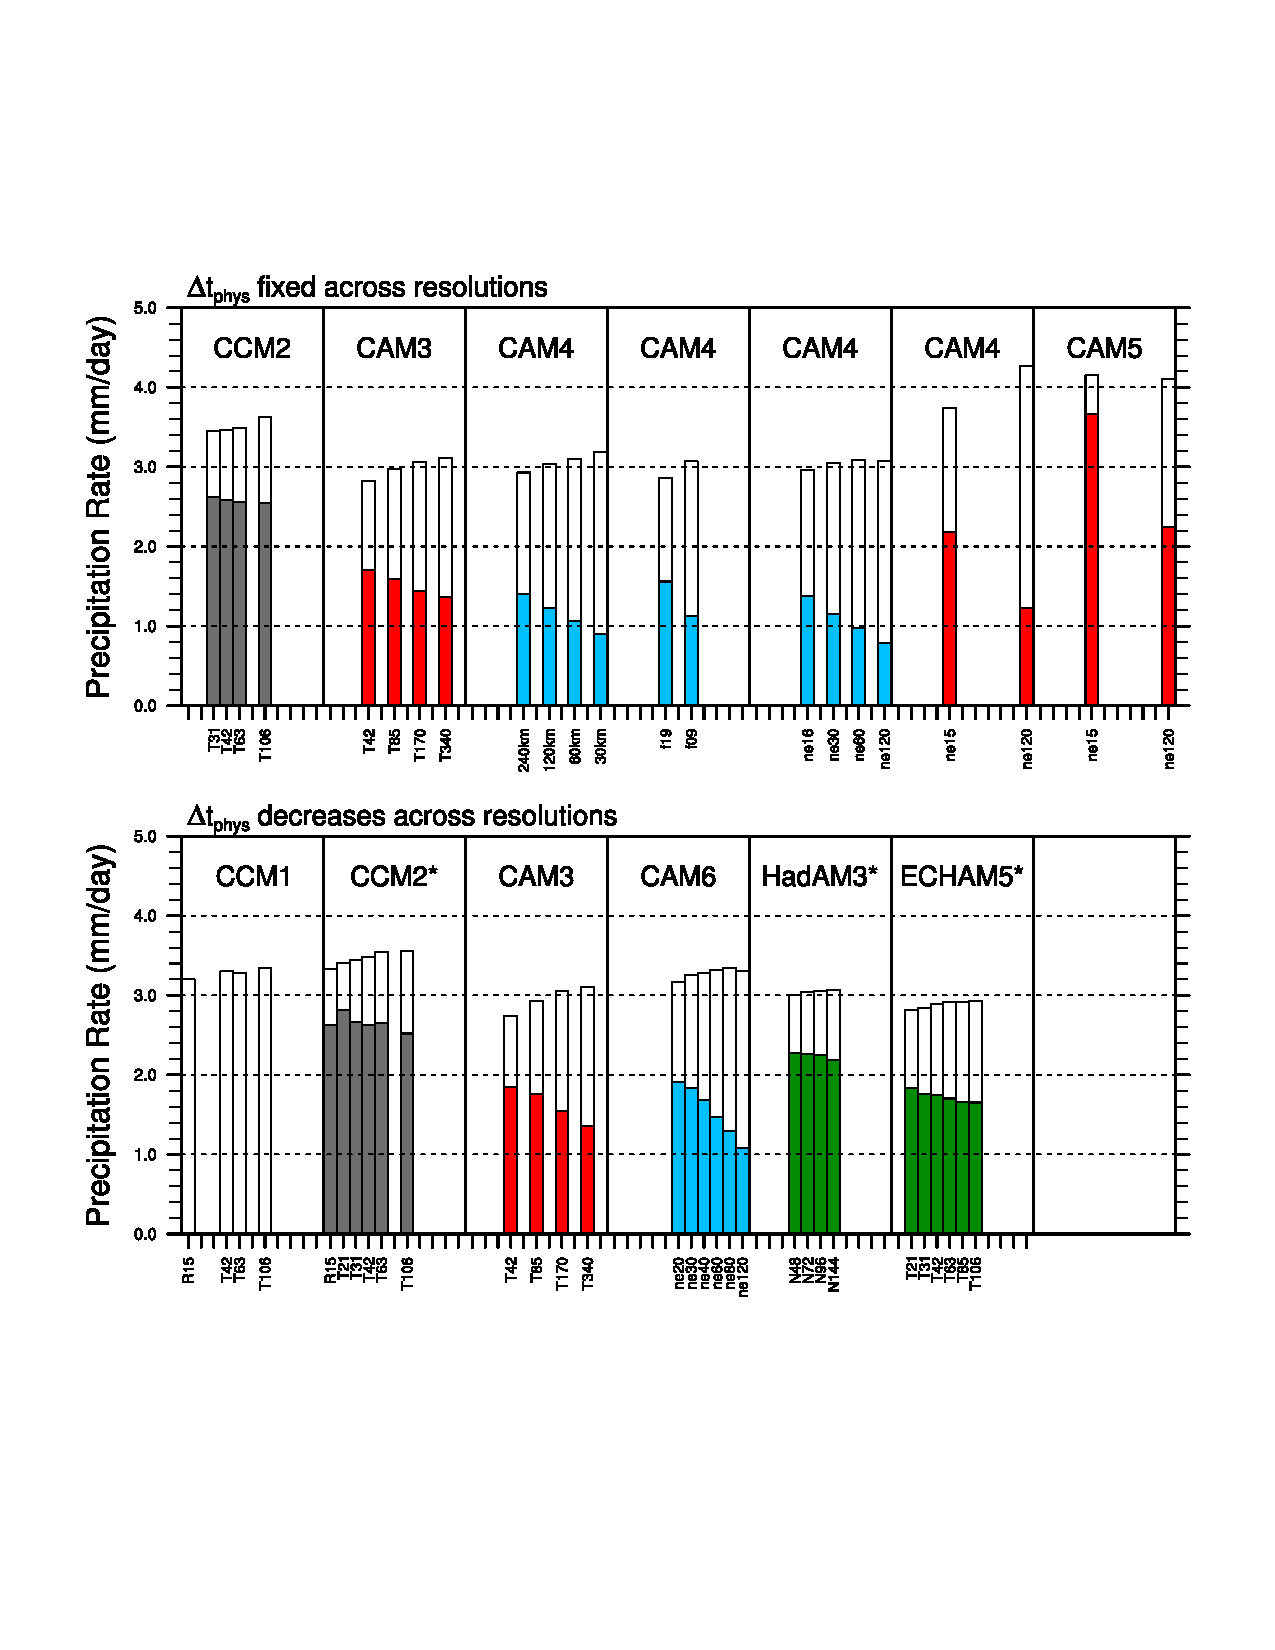
\includegraphics[width=20pc,angle=0]{figs/cam-history.pdf}\\
\end{center}
\caption{Bar-graph of the convective (solid) and stratiform (white) climatological precipitation rates in prior CAM/CCM convergence studies. Each window contains a single convergence study, with identical x-axis; the approximate grid resolution. Colors indicate the model configuration; January ensemble (black) and aqua-planet configurations with SST profiles $QOBS$ (blue) and $CNTL$ (red) after \cite{NH2000ASL}. Studies included in this figure are \cite{KW1991JGR} (CCM1), \cite{WETAL1995CD} (CCM2), \cite{W2008TELLUS} (CAM3), \cite{RETAL2013JCLIM,ZetAl2014JCb,HR2017JCLIM} (CAM4), \cite{ZetAl2014JCb} (CAM5) and this study (CAM6). CCM2* refers to the modified parameter experiment of \cite{WETAL1995CD}, where parameters vary with resolution to reduce the dependence of cloud fraction on resolution.}
\label{fig:cam-history}
\end{figure}

In this study, a convergence experiment using CAM, version 6 (CAM6; \url{https://ncar.github.io/CAM/doc/build/html/users_guide/index.html}) is carried out and analyzed in detail. It is shown that the resolution sensitivity of vertical velocities are well described with $n=-1$ in equation~\eqref{eq:alpha}, provided $\Delta t_{phys}$ is defined in a way that avoids large truncation errors across resolutions. The reduction in convective precipitation rates with resolution in CAM6 is shown to result from the greater magnitude subsiding motion, creating a more stable atmosphere in which the criterion for parameterized convection occurs less often. The increase in stratiform precipitation rates with resolution is shown to result more directly from the increase in vertical velocities, by increasing moisture fluxes through the cloud base level. The feedback of the resolved vertical motion on the physics indicates that the root cause of resolution sensitivity in CAM arises from the sensitivity of resolved dynamical modes to native grid resolution. Section 2 describes CAM6 and the details of the convergence experiment. Section 3 contains a thorough analysis of the CAM6 simulations and Section 4 provides some discussion and conclusions.

\section{Methods}

\subsection{Dynamical Core}

This study uses the spectral-element dynamical core option of Community Atmosphere Model \citep[CAM-SE;][]{DetAl2012IJHPCA}, coupled with a mass conserving, semi-Lagrangian advection method for accelerated multi-tracer transport \citep[CSLAM;][]{LTOUNGK2017MWR}, and dry-mass vertical coordinate with comprehensive treatment of moisture and energy \citep{LetAl2018JAMES}. The dry dynamics are solved using the high-order, momentum, mass and energy conserving spectral element method \citep{TF2010JCP}, with the elements defined by a cubed-sphere grid. The notation for the horizontal grid resolution is an `$ne$' followed by the number of elements making up an edge of one cubed-sphere face, e.g., $ne30$. Hyper-viscous $\nabla^{4}$ explicit numerical dissipation is applied to temperature, dry pressure thickness, rotational and divergent winds \citep{LetAl2018JAMES}. CSLAM tracer transport uses a finite volume grid constructed from the cubed-sphere of elements, and contains the same degrees of freedom as the dry dynamics.

\subsection{Physical Parameterizations}

The physics are evaluated on the finite-volume CSLAM grid, and the tendencies mapped back to the spectral element grid. The coupled system, referred to as CAM-SE-CSLAM, conserves energy, mass and preserves linear correlations between two reactive species to within machine precision \citep{HL2018MWR}. A coarser physics grid, containing $\frac{5}{9}$ fewer degrees of freedom than the dynamical core grid is also available as part of the CAM-SE-CSLAM package \citep{HETAL2019JAMES}. This lower-resolution physics grid is used in this study, but only as a member of a perturbed parameter ensemble and not in the default convergence experiment. The dynamics time-step is subcycled within a longer physics time-step $\Delta t_{phys}$, and the temperature and momentum increments from the physics are divided by the number of subcycles and added to the dynamical core at the beginning of each subcycle. The full moisture increment from the physics is applied only at the start of the first subcycle to conserve tracer mass \citep[$ftype=2$ option in][]{LW2019JAMES}.

The simulations use the CAM6 physics package. The Cloud Layers Unified by Binormals \citep[CLUBB][]{GETAL2002JAS,BOG2013JCLIM} is an assumed filtered density function \citep{G1992JFM} high-order closure model that handles shallow convection, planetary boundary layer mixing and cloud macrophysics. The macrophyiscs are coupled with a two-moment bulk cloud microphysics scheme with prognostic precipitation \citep{MG2}, and microphysics are coupled with a three mode Modular Aerosol Model \citep{MAM}. The combined macrophysics/microphysics routines generate stratiform precipitation from stratiform clouds. Deep convection is parameterized using a quasi-equilibrium mass flux scheme \citep{ZM1995AO} and an entraining plume model \citep[referred to as the dilute convective available potential energy, or {\em{dilute CAPE}} hereafter;][]{RB1992JAS, NRJ2008JC} is used as a convective trigger (convection occurs if dilute CAPE $\geq 70$ J/kg), and for closing the mass fluxes in the cloud ensemble. The deep convection scheme also parameterizes convective momentum transport \citep{RR2008JC}.

\subsection{Experimental Design}
 
The convergence experiment is performed in an aqua-planet configuration \citep{NH2000ASL,MWO2016JAMES}, an all ocean planet with fixed, zonally symmetric sea surface temperatures modeled after present day Earth \citep[$QOBS$ in][]{NH2000ASL}. The aqua-planets are in a perpetual equinox, and aerosols are largely absent from the simulations. Each simulation is ran for one simulated year. Six different horizontal grids are used in this study, which are provided in Table~\ref{tbl:table1}. In addition to the six simulations used in the convergence experiment, an ensemble of 24 simulations containing different model parameters (e.g., using the lower resolution physics grid) and across different resolutions are ran for one year in order to increase confidence in the assessment of resolution sensitivity in this study. All analyses exclude the first month of the simulations, and are computed on their native grids unless otherwise stated.

 \begin{table*}
 \caption{Experimental design and global mean climatologies. $\Delta x$ refers to the average equatorial grid-spacing.}
 \centering
 \scriptsize
 \begin{tabular}{lcccccc}
   \hline
   Variable & $ne20$ & $ne30$ & $ne40$ & $ne60$ & $ne80$ & $ne120$ \\ 
   \hline
   $\Delta x$ (km) & 166.8 & 111.2 & 83.4 & 55.6 & 41.7 & 27.8 \\
   $\nu$ ($m^4/s$) & $1.5 \times 10^{15}$ & $4.0 \times 10^{14}$ & $1.5 \times 10^{14}$ & $4.0 \times 10^{13}$  & $1.5 \times 10^{13}$ & $4.0 \times 10^{12}$\\
    $\Delta t_{phys}$ (s) & 2700 & 1800 & 1350 & 900 & 675 & 450 \\
   Total Cloud Fraction & 0.844 & 0.835 & 0.824 & 0.810 & 0.804 & 0.800 \\ 
   Total Precipitable Water (mm) & 23.31& 23.01 & 22.62 & 22.25 & 21.93 & 21.72 \\
   Convective Precipitation (mm/day) & 1.91 & 1.83 & 1.68 & 1.47 & 1.29 & 1.08 \\
   Stratiform Precipitation (mm/day) & 1.26 & 1.42 & 1.60 & 1.85 & 2.05 & 2.22 \\      
 \hline
 \end{tabular}
 \label{tbl:table1}
 \end{table*}

The horizontal hyper-viscosity operators $\nu$ vary with resolution after \cite{HETAL2019JAMES}, also provided in Table~\ref{tbl:table1}. The values of $\nu$ are a factor 2.5 greater for divergence damping and are not shown. $\Delta t_{phys}$ is chosen to scale with resolution, in proportion to the grid spacing,
\begin{equation}
\Delta t_{phys} = \Delta t_{phys,0} \times \frac{n_{e,0}}{n_e}~s,\label{eq:dt-scale}
\end{equation}
where $\Delta t_{phys,0}$ is taken to be the standard $1800$ s used in CAM-SE-CSLAM for the standard climate resolution, $n_{e,0} = 30$ (equivalent to an average equatorial grid spacing $\Delta x = 111.2$km). This scaling was chosen to avoid large time-truncation errors in a rising moist bubble test \citep[Appendix A in][]{HETAL2019JAMES}, and it is understood that this choice of $\Delta t_{phys}$ will likely lead to greater resolution sensitivity \citep{W2008TELLUS}. The convective time-scale in the deep convection scheme is fixed at 3600 s in all simulations.
 
 \section{Results}

Table~\ref{tbl:table1} provides some globally averaged, climatological metrics for the CAM6 convergence experiment, commonly published in CAM/CCM convergence studies. Total precipitable water, total cloud fraction and deep convective precipitation rate decreases, while stratiform precipitation increases, monotonically with resolution (also shown in Figure~\ref{fig:cam-history}). Resolution sensitivity in CAM6 is similar to all prior versions of the model. 

\subsection{Vertical Velocities and Resolution}

\begin{figure}
\begin{center}
\noindent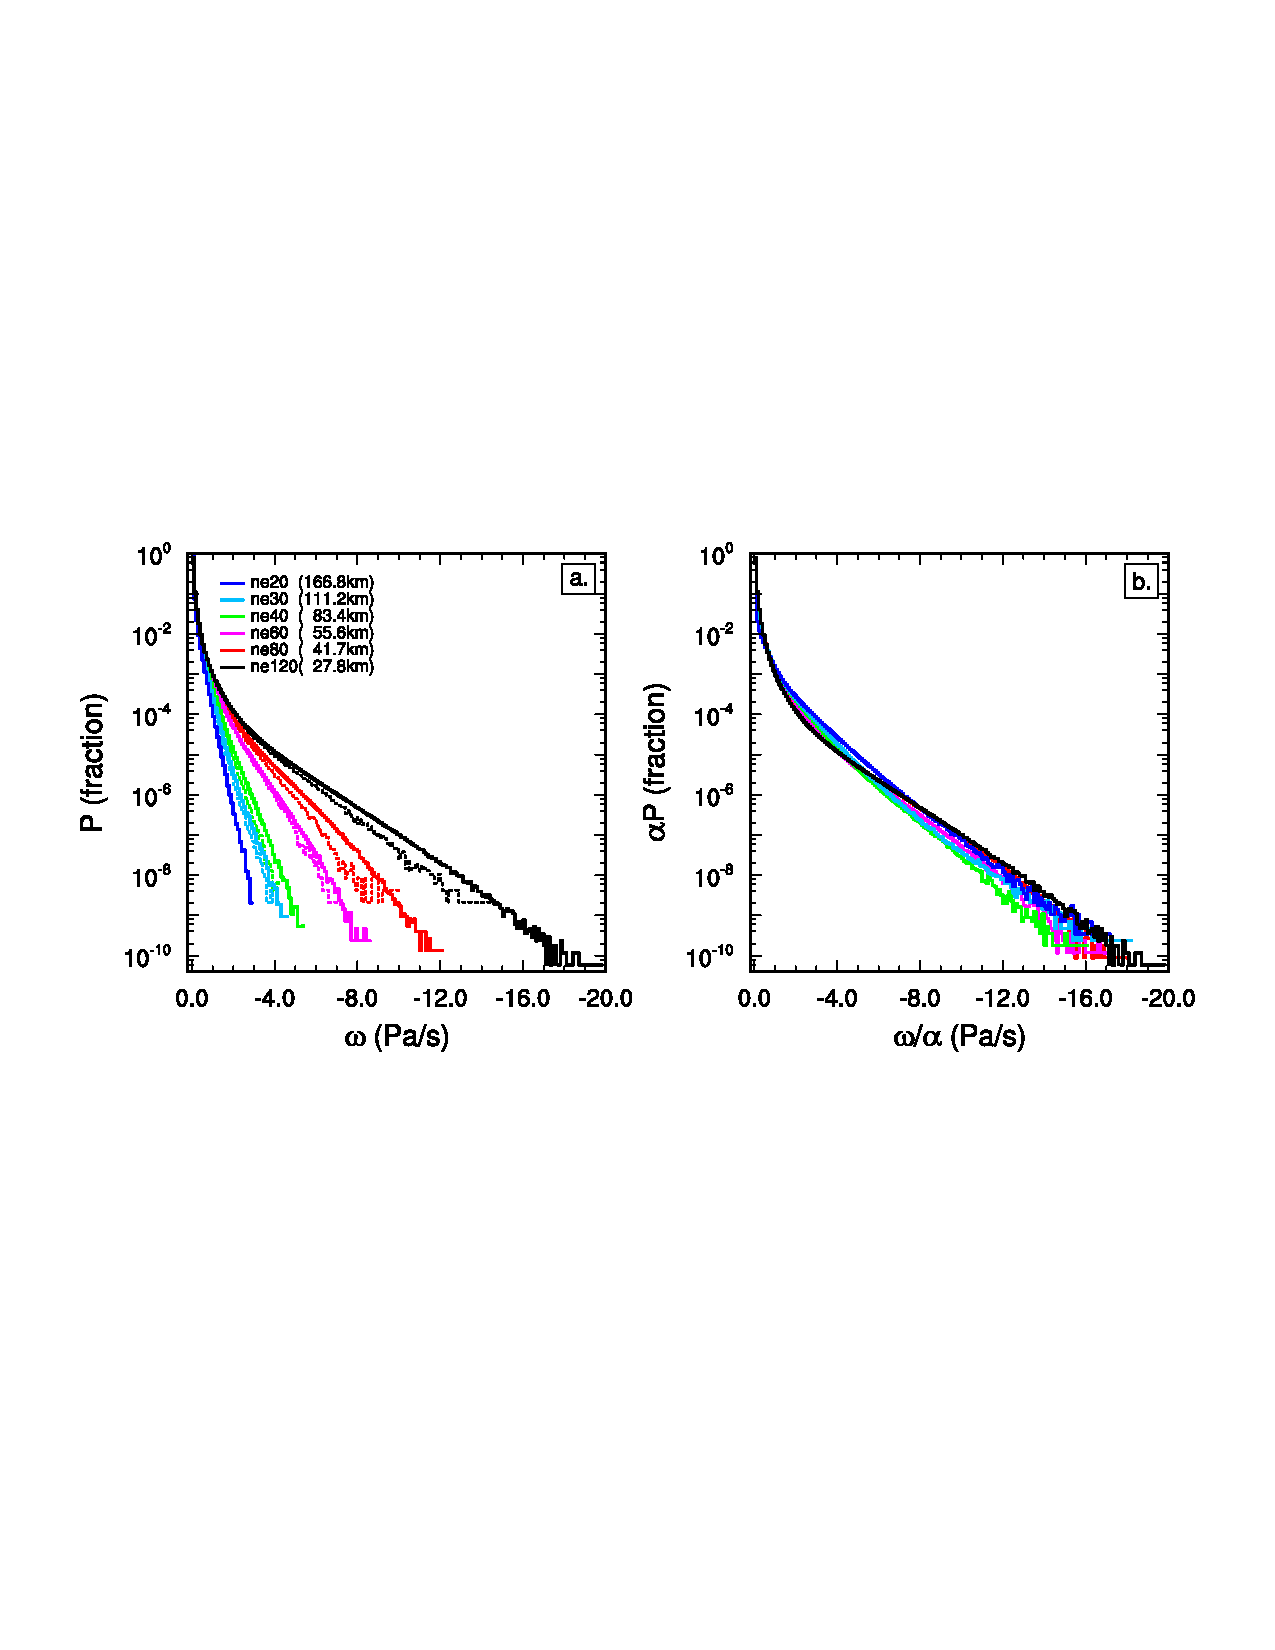
\includegraphics[width=20pc,angle=0]{figs/temp_2pdf.pdf}\\
\end{center}
\caption{Probability density distribution of the upward vertical pressure velocities $\omega$ computed everywhere in the model from six-hourly output over the entirety of the year-long simulations. (a) Values on their native grid (solid) and values remapped to the $ne20$ grid (dotted), (b) values on their native grid, scaled to the $ne120$ resolution using a power law exponent $n=-1$ in equation~\ref{eq:alpha}.}
\label{fig:2pdf}
\end{figure}

The probability density function (PDF) of negative, or upward vertical pressure velocities $\omega$ in the aqua-planets is provided in Figure~\ref{fig:2pdf}a. The magnitude of upward $\omega$ increases monotonically with resolution, with positive, or downward $\omega$ behaving similarly (not shown). This monotonic increase in the magnitude of $\omega$ is evident even after remapping all the model output to a common grid ($ne20$; dotted curves in Figure~\ref{fig:2pdf}a).

The PDF's may be scaled to the highest-resolution resolution grid through $P(\omega)_s = \alpha P (\omega / \alpha)$, where $\alpha$ is the scale factor from equation~\ref{eq:alpha}, and setting $\Delta x_0$ to the $ne120$ grid-spacing. Figure~\ref{fig:2pdf}b shows the scaled PDF's for power law exponent $n=-1$ in equation~\ref{eq:alpha}. The scaled PDF's all collapse onto the high-resolution reference, indicating that the power-law exponent $n=-1$ explains to first-order the variation in vertical velocity with resolution in the aqua-planet simulations. 

Changes to the vertical velocity field can be further understood through decomposing the mass weighted vertical mean $ \langle \omega \rangle$ into upward and downward components,
\begin{equation}
\langle \omega \rangle =\langle f_{u} \rangle \, \langle \omega_{u} \rangle + \langle f_{d} \rangle \, \langle \omega_{d} \rangle, \label{eq:omega}
\end{equation}
where $\langle f_x \rangle$ and $\langle \omega_x \rangle$ refers to the vertical mass fraction $ \left( \frac{\int dp_x}{\int dp} \right)$ and the $x$ component of the mass weighted vertical mean of $\omega$ $ \left( \frac{\int \omega_x dp_x}{\int dp_x} \right)$, respectively, subscript $u$ refers to upward motion and $d$, downward motion.

The global mean, climatological components $\langle f_{u} \rangle \, \langle \omega_{u} \rangle$ and $\langle f_{d} \rangle \, \langle \omega_{d} \rangle$ are provided in Figure~\ref{fig:2panel}a,b for the aqua-planet simulations. The magnitude of both $\langle f_{u} \rangle \, \langle \omega_{u} \rangle$ and $\langle f_{d} \rangle \, \langle \omega_{d} \rangle$ increase monotonically with resolution, and are equal and opposite, which is a requirement of mass conservation in the model and a convenient check of the calculation. While $\langle f_{d} \rangle$ is about 25\% larger than $\langle f_{u} \rangle$ in all simulations, the vertical mass fractions vary by only few percent with resolution, and so the monotonic behavior of $\langle f_{x} \rangle \, \langle \omega_{x} \rangle$ with resolution is primarily from variations in $ \langle \omega_{x} \rangle$ (not shown).

\begin{figure}
\begin{center}
\noindent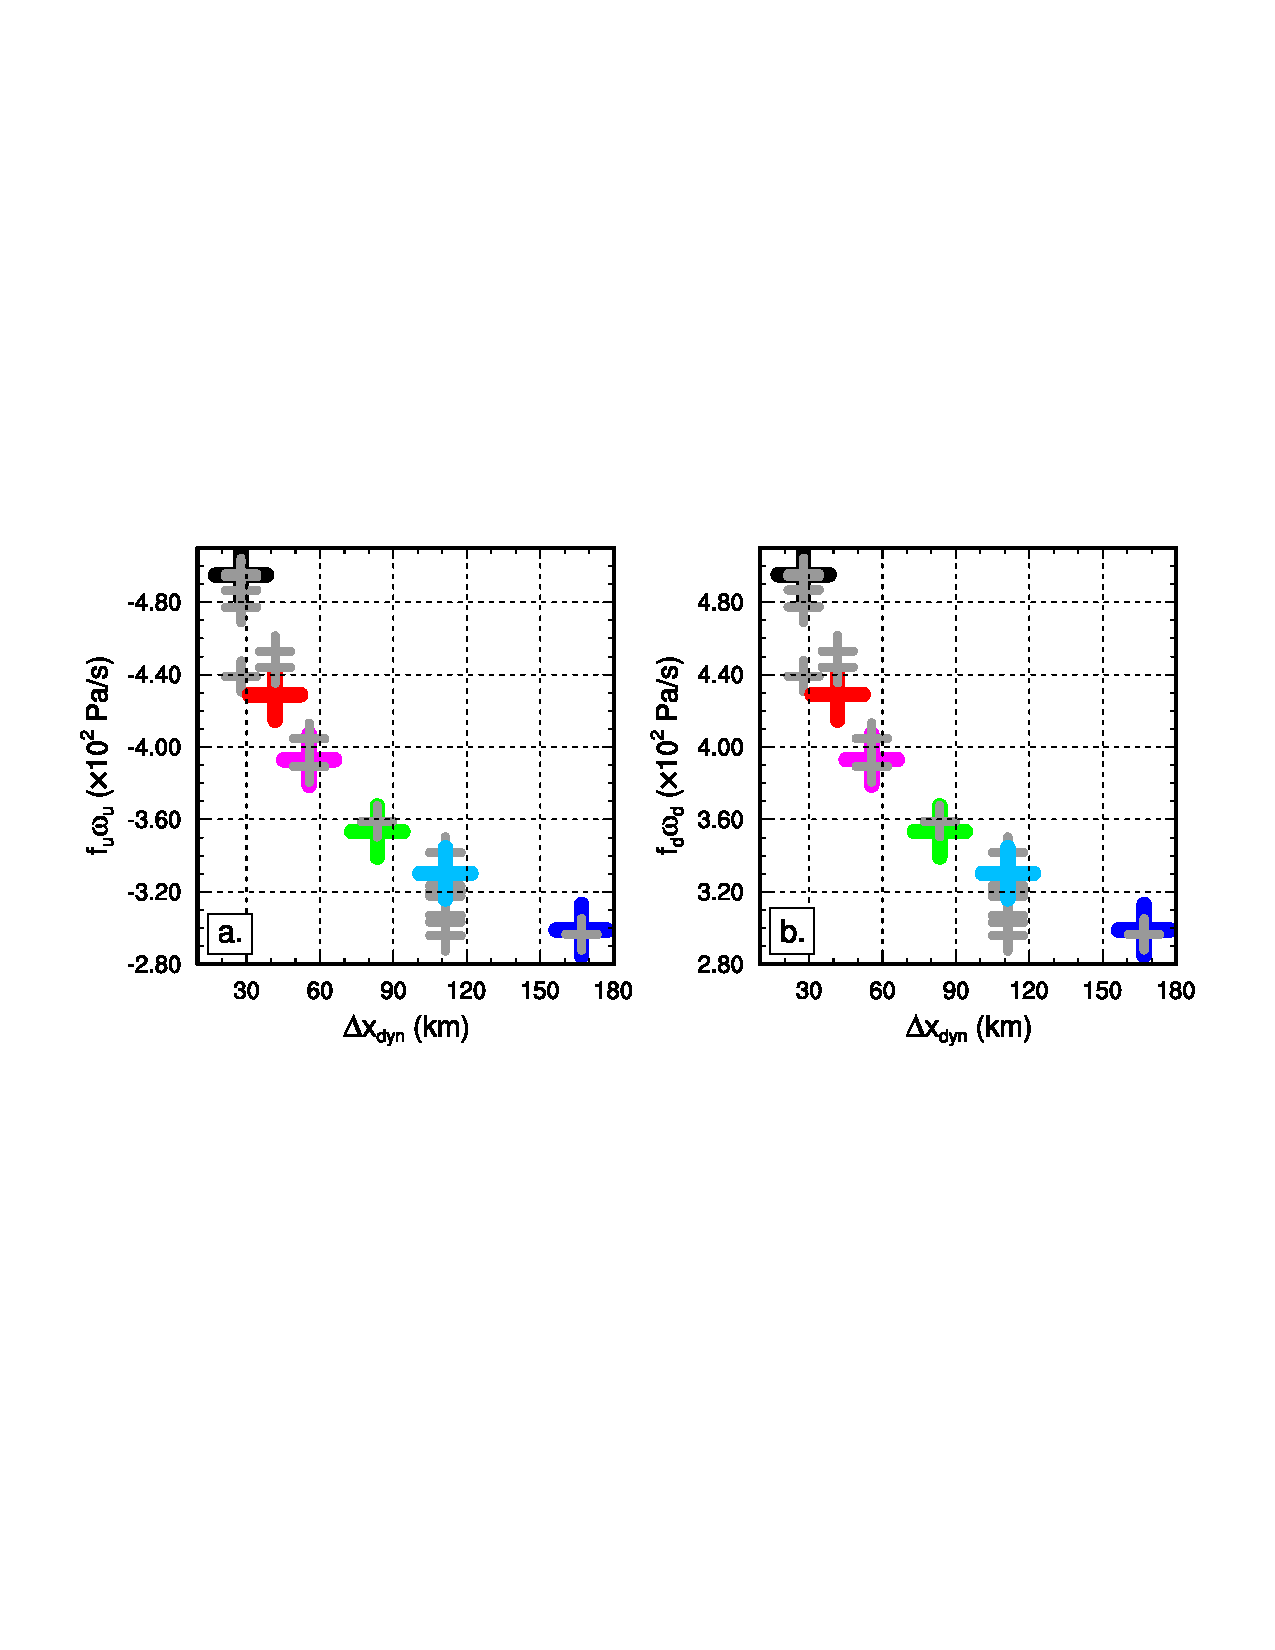
\includegraphics[width=20pc,angle=0]{figs/temp_diags_2panel.pdf}\\
\end{center}
\caption{Components of the climatological, global mean vertical pressure velocity, (a) $\langle f_{u} \rangle \langle \omega_{u} \rangle$ and (b) $\langle f_{d} \rangle \langle \omega_{d} \rangle$. Grey crosses are for the 24 member perturbed parameter ensemble.}
\label{fig:2panel}
\end{figure}

\subsection{Vertical Velocities and Deep Convective Precipitation}

The large increase in magnitude of the upward and downward vertical velocities with resolution may be expected to impact the behavior of other model components. Curiously, there is an excellent negative correlation (Pearson's R-value = 0.99, N = 27) between the global mean, climatological $\langle f_{d} \rangle \, \langle \omega_{d} \rangle$ and a measure of the activity of the \cite{ZM1995AO} deep convection scheme (referred to as the {\em{ZM scheme}} hereafter), global mean, climatological $FREQZM$ (Figure~\ref{fig:corr}). At any grid-point and time-step, $FREQZM$ is a binary variable: one if the ZM scheme is active, zero if it is not. Time mean $FREQZM$ is therefore the fraction of the model time that the ZM scheme is triggered, i.e., dilute CAPE exceeds $\geq 70$ J/kg. The regression indicates that model simulations with greater subsidence also have less convective activity.

\begin{figure}
\begin{center}
\noindent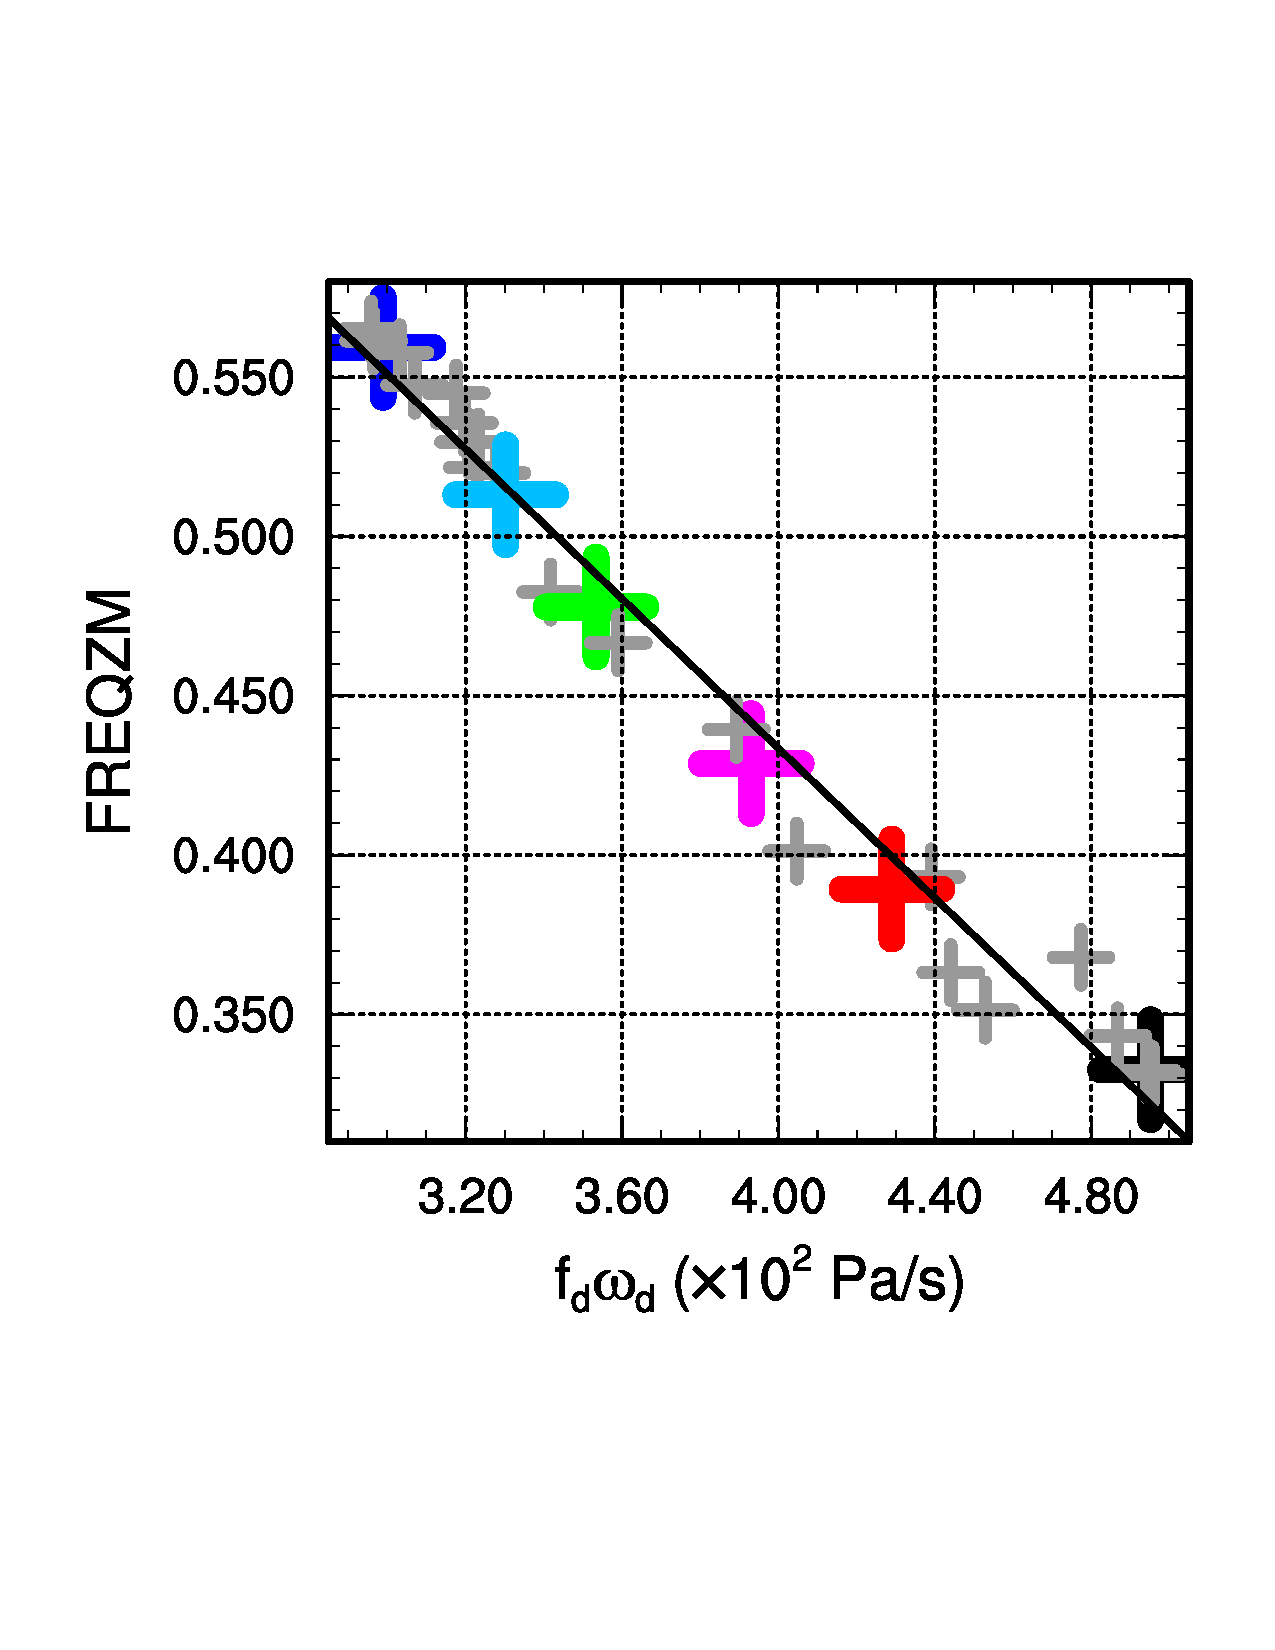
\includegraphics[width=20pc,angle=0]{figs/temp_diags_corr.pdf}\\
\end{center}
\caption{Scatter plot of global mean, climatological $\langle f_{d} \rangle \langle \omega_{d} \rangle$ and FREQZM, and the fitted linear regression which has a Pearson's R-value = 0.99, using all 27 simulations. Grey crosses are for the 24 member perturbed parameter ensemble runs.}
\label{fig:corr}
\end{figure}

To further understand this relationship, a logistic regression between $\langle f_{d} \rangle \langle \omega_{d} \rangle$ and $FREQZM$ is performed for each grid column within each of the simulations. Logistic regression uses an iterative method to fit a continuous variable predictor, $x$ to a binary predictand $p$ using the exponential \citep{WILKSBOOK},
\begin{equation}
p = \frac{exp{[b_0 + b_1 x]}}{1 + exp{[b_0 + b_1 x]}}, \label{eq:eq6-3}
\end{equation}
where $b_0$ and $b_1$ are the shape parameters of the exponential. The predictor is the instantaneous $\langle f_{d} \rangle \langle \omega_{d} \rangle$ of a grid column, and the predictand the binary $FREQZM$. The assumption is then that subsidence is the independent variable, which the authors believe is reasonable since the environment of subsiding regions is generally more stable than its surroundings, and the ZM scheme is modulated by a stability calculation, dilute CAPE. Grid column regressions that are statistically significant at the $95\%$ level using a log-likelihood test \citep{WILKSBOOK} are retained for analysis. Since the aqua-planets have zonally symmetric boundary conditions, there is a zonally varying structure in the goodness of fit (R-value) and parameter $b_1$ (hereafter referred to as the sensitivity parameter; Figure~\ref{fig:4zonal}a,b).

\begin{figure}
\begin{center}
\noindent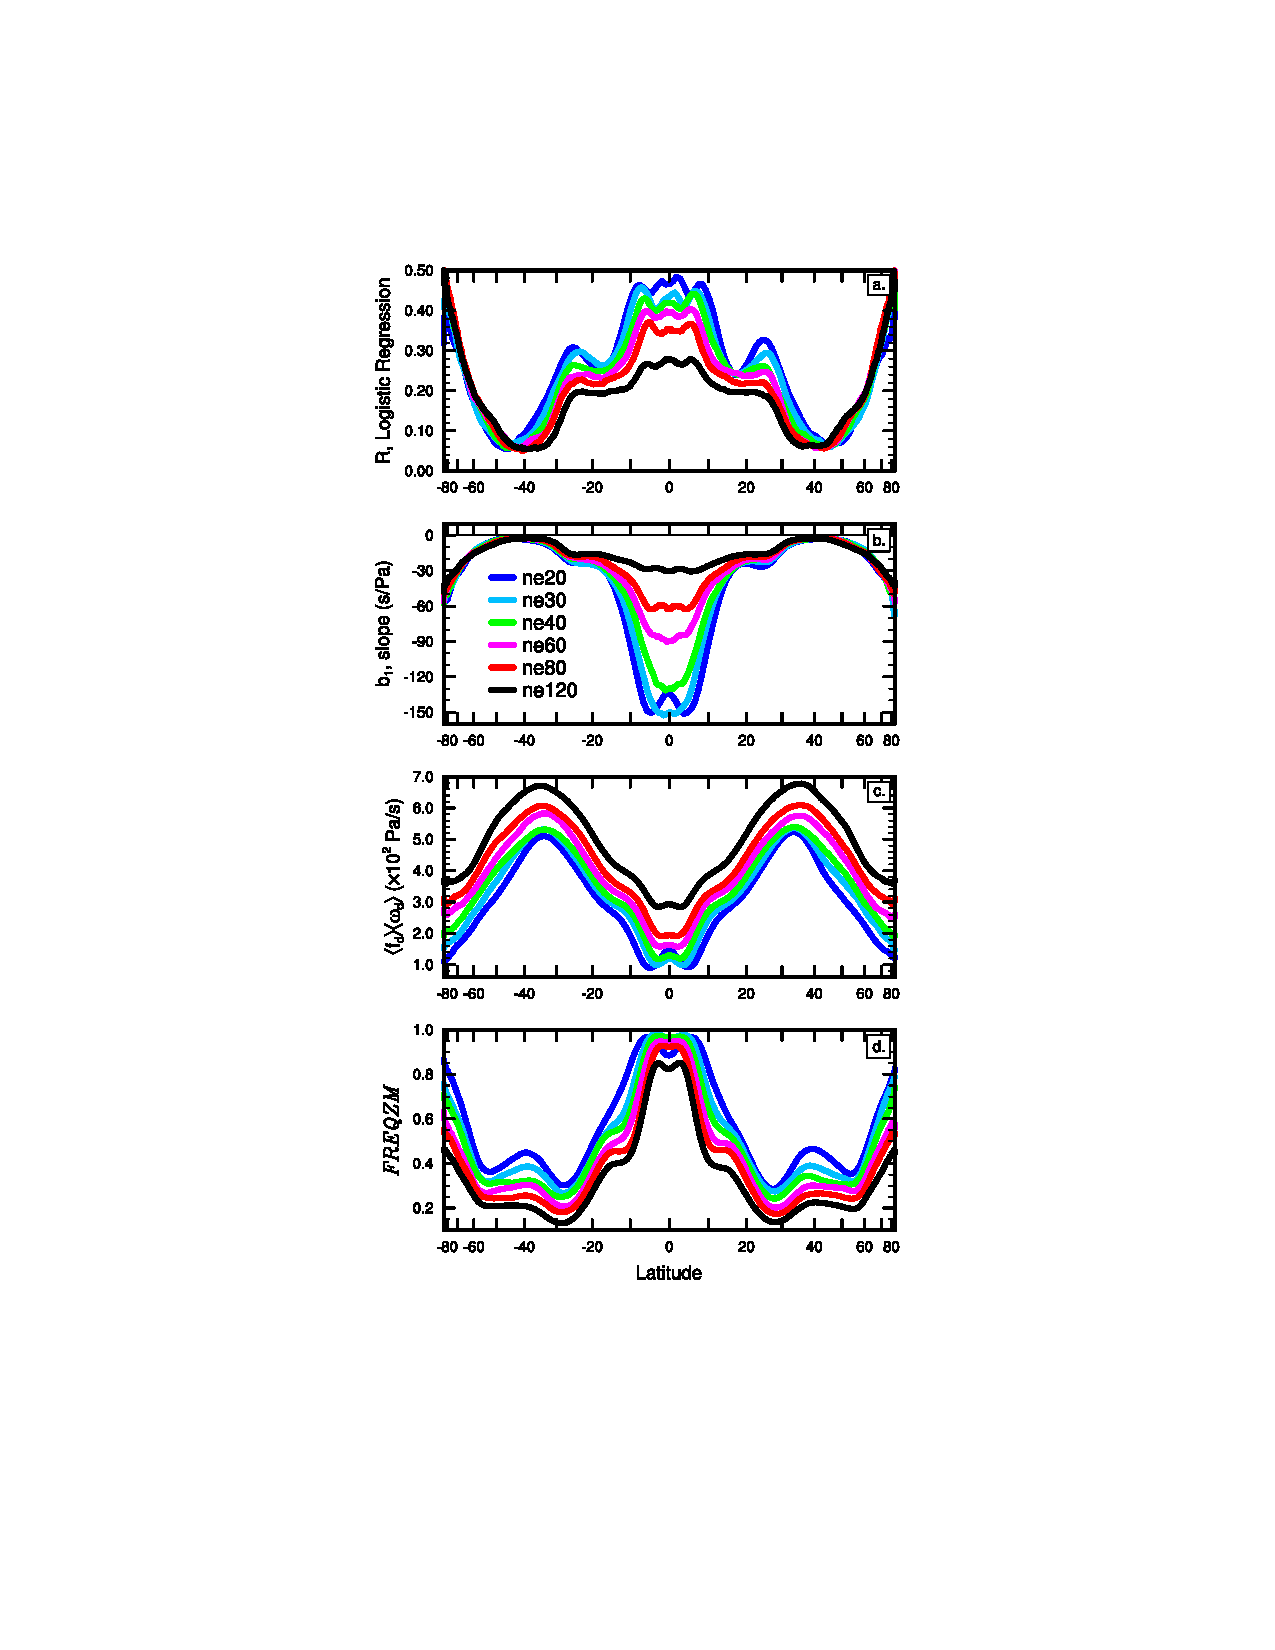
\includegraphics[width=14pc,angle=0]{figs/temp_4zonal.pdf}\\
\end{center}
\caption{Zonal mean (a) R-values and (b) sensitivity parameter in the logistic regression, (c) climatological surface latent heat fluxes and (d) drizzle fraction.}
\label{fig:4zonal}
\end{figure}

The zonal mean R-values indicate the greatest goodness of fit in the $\pm 10^{\circ}$ latitude band, hereafter referred to as the deep tropics. In this region, the sensitivity parameter is large and negative (Figure~\ref{fig:4zonal}b), consistent with the idea that subsiding motion stabilizes the environment and actively depresses dilute CAPE and the activity of the ZM scheme in the simulations. The sensitivity parameter becomes less negative in the deep tropics with resolution, likely due to the greater magnitude $\langle f_{d} \rangle \langle \omega_{d} \rangle$ with resolution, which requires a lower sensitivity parameter to predict the binary $FREQZM$. The R-values generally decrease with resolution indicating that there is degradation in the relationship with resolution.

Table~\ref{tbl:table2} shows the fractional contribution of the deep tropics to the climatological, global mean change in convective precipitation with resolution. This is a reflection of changes in the partitioning of the Intertropical Convergence Zone (ITCZ) from convective to stratiform precipitation with resolution. The table indicates that a majority ($60-70 \%$) of the reduction in convective precipitation with resolution is from changes within the deep tropics (except in going from $ne20$ to $ne30$, where convective precipitation rates increase due to a wide double-ITCZ in the $ne20$ run that spans well outside of $\pm 10^{\circ}$ latitude, but which is contained within $\pm 10^{\circ}$ latitude in the $ne30$ run). Expanding the latitude boundaries marginally to $\pm 15^{\circ}$, roughly $75\%$ of the changes in convective precipitation with resolution occurs in this region (again, ignoring $ne30-ne20$; Table~\ref{tbl:table2}). Taken together, the region with the largest change in convective precipitation with resolution is also the region where the logistic regression indicates that subsiding motion is most skillful at depressing the activity of the convection scheme.

 \begin{table}
 \caption{Fractional contribution of latitude bands $\pm 10^{\circ}$ and $\pm 15^{\circ}$ to changes in global mean precipitation with resolution. The grid headers refer to differences with respect to the next lowest grid resolution, e.g., $ne30 = ne30-ne20$, $ne40=ne40-ne30$, etc... All differences are computed after remapping the data to the $ne20$ grid.}
 \centering
 \scriptsize
 \begin{tabular}{lcccccc}
   \hline
   Variable & $ne30$ & $ne40$ & $ne60$ & $ne80$ & $ne120$ \\ 
   \hline
   $\pm 10^{\circ}$ ($17.6\%$ of global area) \\
   Convective Precipitation & -0.58 & 0.62 & 0.66 & 0.72 & 0.70 \\
   Stratiform Precipitation & 0.55 & 0.63 & 0.69 & 0.67 & 0.41 \\ 
   \hline
   $\pm 15^{\circ}$ ($25.8\%$ of global area) \\
   Convective Precipitation & 0.22 & 0.75 & 0.73 & 0.79 & 0.72 \\
   Stratiform Precipitation & 0.46 & 0.64 & 0.71 & 0.70 & 0.49 \\      
 \hline
 \end{tabular}
 \label{tbl:table2}
 \end{table}

To estimate the dilute CAPE values associated with subsiding motion in the deep tropics, temperature and moisture profiles are conditionally sampled depending on whether $\langle \omega \rangle$ is positive or negative, indicating predominantly subsiding or ascending grid columns. The time mean temperature and moisture profiles of subsiding and ascending regions are then used to compute the dilute CAPE used in the ZM scheme, offline. Figure~\ref{fig:cape}a shows the dilute CAPE values associated with mean conditions for ascending, descending and all grid columns in the deep tropics, with resolution. Ascending regions are associated with larger values of dilute CAPE ($>180$ J/kg) relative to subsiding regions ($<110$ J/kg), and the dilute CAPE value computed for mean conditions over the entire deep tropics decreases monotonically with resolution, consistent with the reduction in convective activity with resolution. 

The space-time weights associated with ascending and descending grid columns in the deep tropics vary drastically with resolution (Figure~\ref{fig:cape}b). The subsiding (ascending) space-time weights change from $0.32$ ($0.68$) at $ne20$, monotonically increasing (decreasing) with resolution to $0.51$ ($0.49$) in $ne120$. The increasing occurrence of stable, subsiding grid columns with resolution results in a reduction in dilute CAPE for the entire deep tropics, verified by the similar values derived through taking the weighted sum of the ascending/descending CAPE values (grey crosses in Figure~\ref{fig:cape}a).

\begin{figure}
\begin{center}
\noindent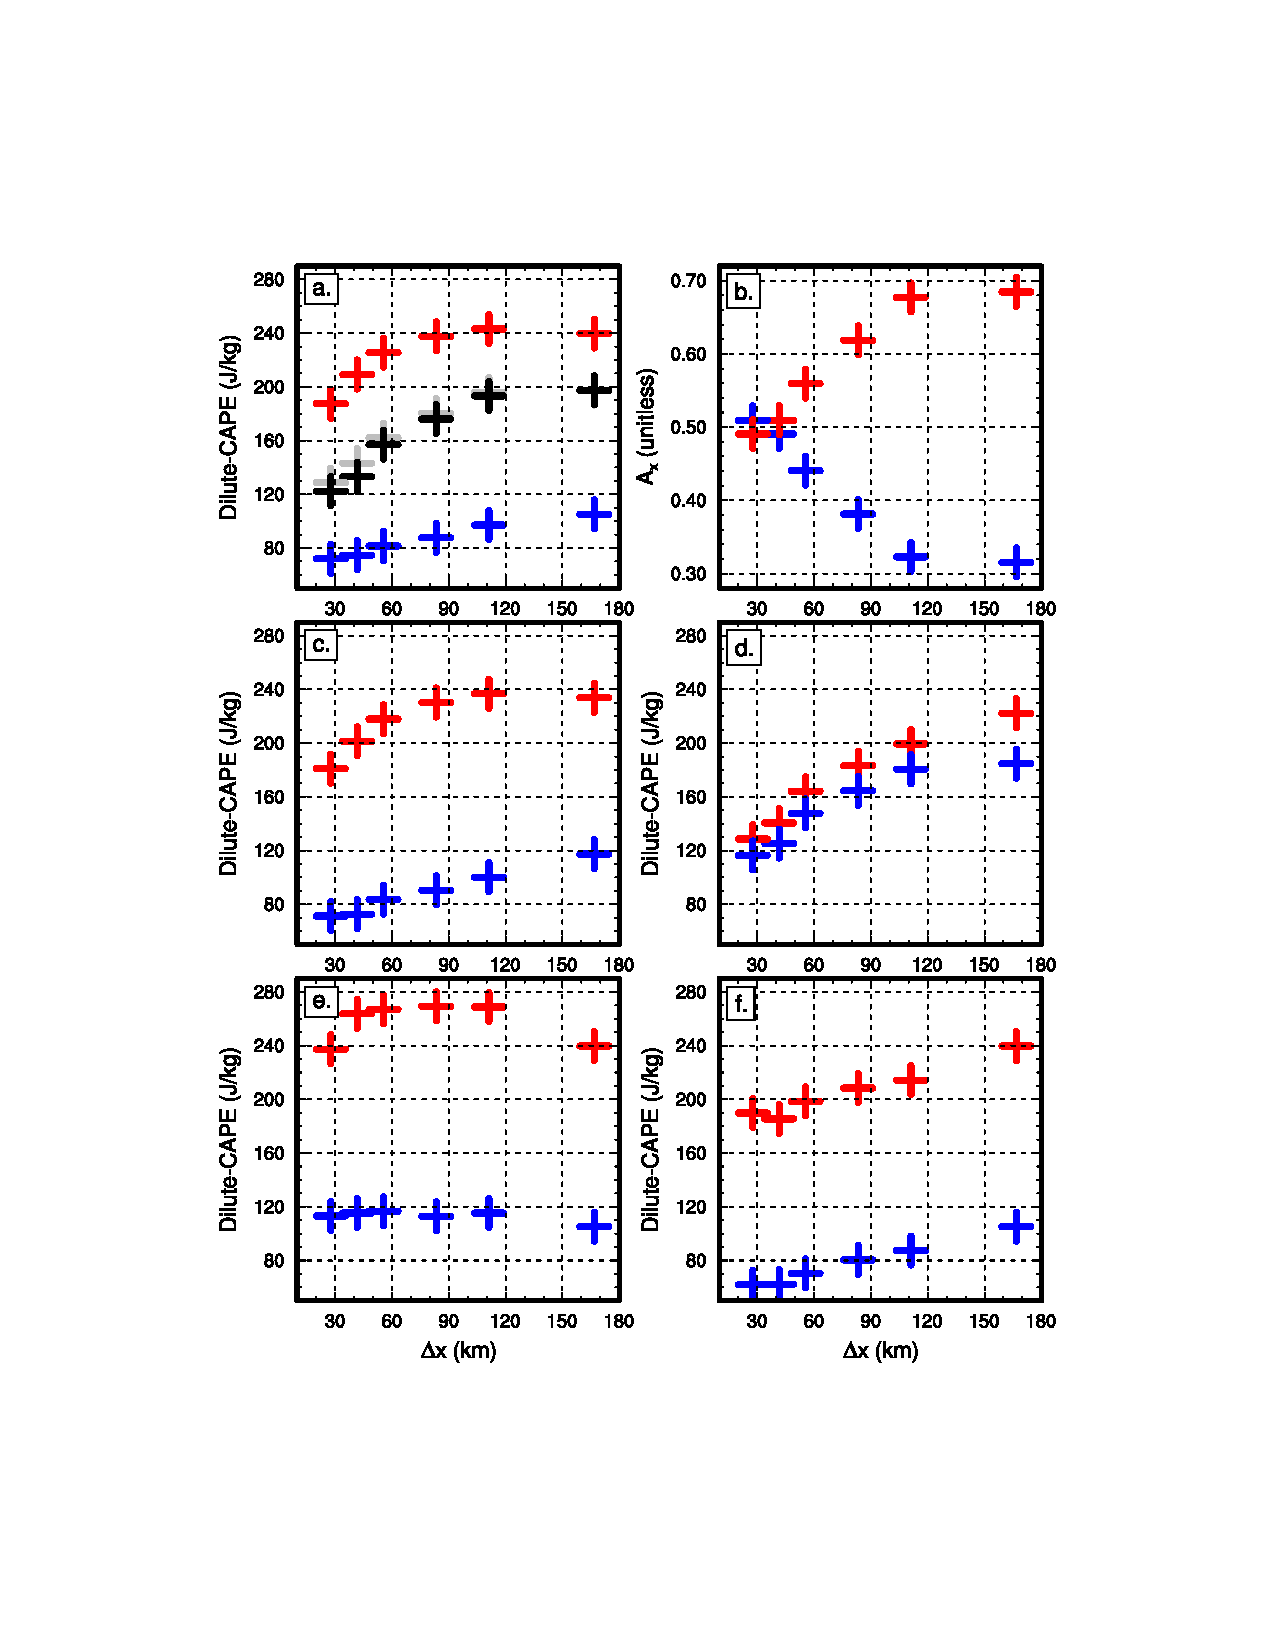
\includegraphics[width=20pc,angle=0]{figs/temp_cape.pdf}\\
\end{center}
\caption{(a) Dilute CAPE computed from time mean temperature and moisture profiles of ascending (red), subsiding (blue) and all grid columns (black) in the deep tropics ($\pm 10^{\circ}$ latitude), and (b) space-time weights of ascending (red) and descending (blue) grid columns in the deep tropics. (c) Dilute CAPE computed for ascending/descending grid columns, but using the mean temperature profile for the entire deep tropics, (d) Same as (c) but using the mean moisture profile for the entire deep tropics. (e) Same as (c) but fixing temperature to the $ne20$ profiles, and (f) same as (d) but fixing moisture to the $ne20$ profile. Grey crosses in (a) are dilute CAPE derived from the sum of the products of space-time weights with the dilute CAPE values of ascending/descending grid columns.}
\label{fig:cape}
\end{figure}

Figure~\ref{fig:profiles} shows the time mean temperature and specific humidity profiles of subsiding grid cells in the deep tropics, expressed as anomalies from the mean temperature and specific humidity of the entire deep tropics. The mean profiles of subsiding regions have an anomalous warming layer in the $600-800$ hPa layer and an anomalous moisture deficit throughout the entire column. This warming and drying patterns is consistent with the effects of subsidence, whose motion adiabatically warms the environment while simultaneously advecting drier conditions aloft downward. Both warming and drying the environment oppose the growth of dilute CAPE through reducing parcel buoyancy; warming the environment relative to the temperature of rising air parcels reduces parcel buoyancy \citep{Z2002JGR}, and mixing drier environmental air into rising air parcels reduces the moisture available to warm parcels through latent heating \citep{RB1992JAS}. 

\begin{figure}
\begin{center}
\noindent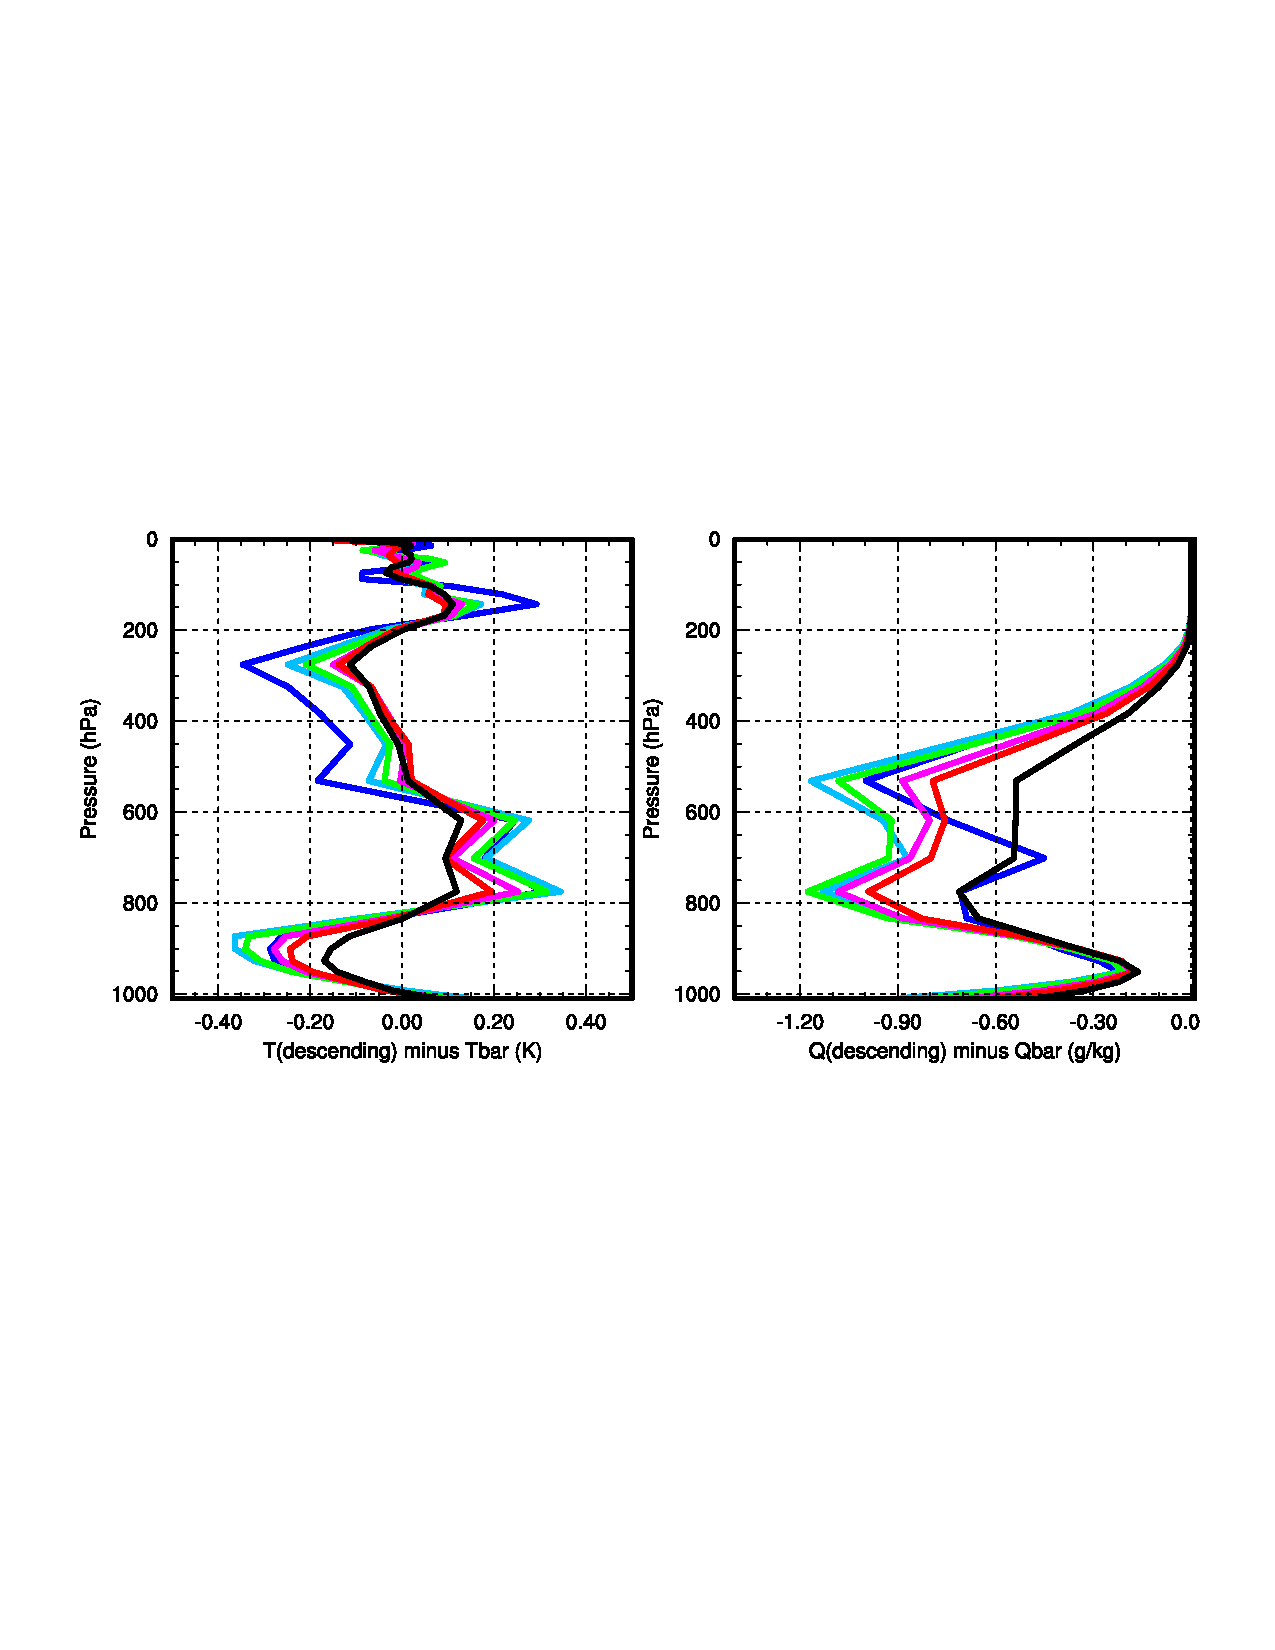
\includegraphics[width=20pc,angle=0]{figs/temp_profiles.pdf}\\
\end{center}
\caption{Time mean (a) temperature and (b) specific humidity profiles of subsiding grid cells in the deep tropics ($\pm 10^{\circ}$ latitude) in the convergence experiment, presented as anomalies from the mean temperature and specific humidity of the entire deep tropics in each simulation.}
\label{fig:profiles}
\end{figure}

{\color{red}{The next three paragraphs need to be condensed into one or two. Working on it.}}

An experiment is carried out to unravel the contributions of warming and drying to dilute CAPE values of subsiding grid columns. Through recomputing dilute CAPE using the mean specific humidity of subsiding regions in the deep tropics, but setting the temperature profile to the mean profile for the entire deep tropics, one can isolate the role of moisture in subsiding regions on the dilute CAPE calculation. Doing the reverse then isolates the role of temperature in subsiding regions on dilute CAPE. 

Figure~\ref{fig:cape}c shows the influence of moisture on the dilute CAPE of subsiding/ascending regions in the deep tropics, and Figure~\ref{fig:cape}d the influence of temperature. To first order, the large spread in dilute CAPE between subsiding and ascending regions is due to the difference in moisture in subsiding and ascending regions, while temperature differences between the two regimes has a smaller, second order influence on the spread of dilute CAPE. A large spread in dilute CAPE between ascending/descending regions is important for maintaining a strong relationship between subsidence and the activity of the ZM scheme. If the model operated more similar to the fixed moisture experiment (Figure~\ref{fig:cape}d), then subsidence would be associated with larger values of dilute CAPE, and less effective at depressing dilute CAPE below the threshold for convection.

The large spread in dilute CAPE of subsiding/ascending regions combined with the large changes in space-time fraction of subsiding/ascending with resolution are responsible for about half of the change in the dilute CAPE computed for the entire deep tropics. There is also a systematic offset of dilute CAPE values in both subsiding/ascending regions with resolution (Figure~\ref{fig:cape}a) that accounts for another half of the resolution sensitivity. To understand whether moisture or temperature changes with resolution are responsible for this behavior, a similar experiment is performed in which dilute CAPE is recomputed at all resolutions, but fixing the moisture profiles to the lowest resolution $ne20$ profile, and then repeated through fixing only the temperature profile to $ne20$ values. Figure~\ref{fig:cape}e,d shows the influence of the change of resolution on moisture, and the change due to temperature, respectively. The calculation shows that temperature changes with resolution are primarily responsible for the other half of the decrease in dilute CAPE in the deep tropics with resolution. 

\subsection{Vertical Velocities and Shallow Convective Precipitation}

AGCMs are known to suffer from a drizzle bias, producing too much light rain relative to observations \citep{D2006JCLIM}. Figure~\ref{fig:4zonal}d shows the fraction of ZM precipitation $\leq 5$ mm/day in the simulations, which stubbornly persists at 70\% in the region between $10^{\circ}-20^{\circ}$ latitude irrespective of resolution. Focusing in on this drizzle region, Figure~\ref{fig:transect} shows two snapshots of $\omega$ in the longitude-pressure plane at  $\sim 18^{\circ}$ latitude in the $ne30$ simulations, overlain by an isoline delineating where the ZM mass fluxes are quite active. The ZM mass fluxes typically only extend up to about the $800$ hPa level, which often occurs with subsiding motion aloft. 

In drizzling regions, there are opposing influences on dilute CAPE, a global maximum in latent heat fluxes (Figure~\ref{fig:4zonal}c), influencing the thermodynamic state of boundary layer parcels and increasing dilute CAPE from below \citep{Z2002JGR}, and subsidence, which opposes dilute CAPE from above. It seems plausible that these two opposing influences on stability translates into small values of dilute CAPE, but for drizzle to occur, still large enough to trigger the ZM scheme. The ZM scheme, properly a deep convection scheme, is operating as a shallow convection scheme in the $10^{\circ}-20^{\circ}$ latitude region.

\begin{figure}
\begin{center}
\noindent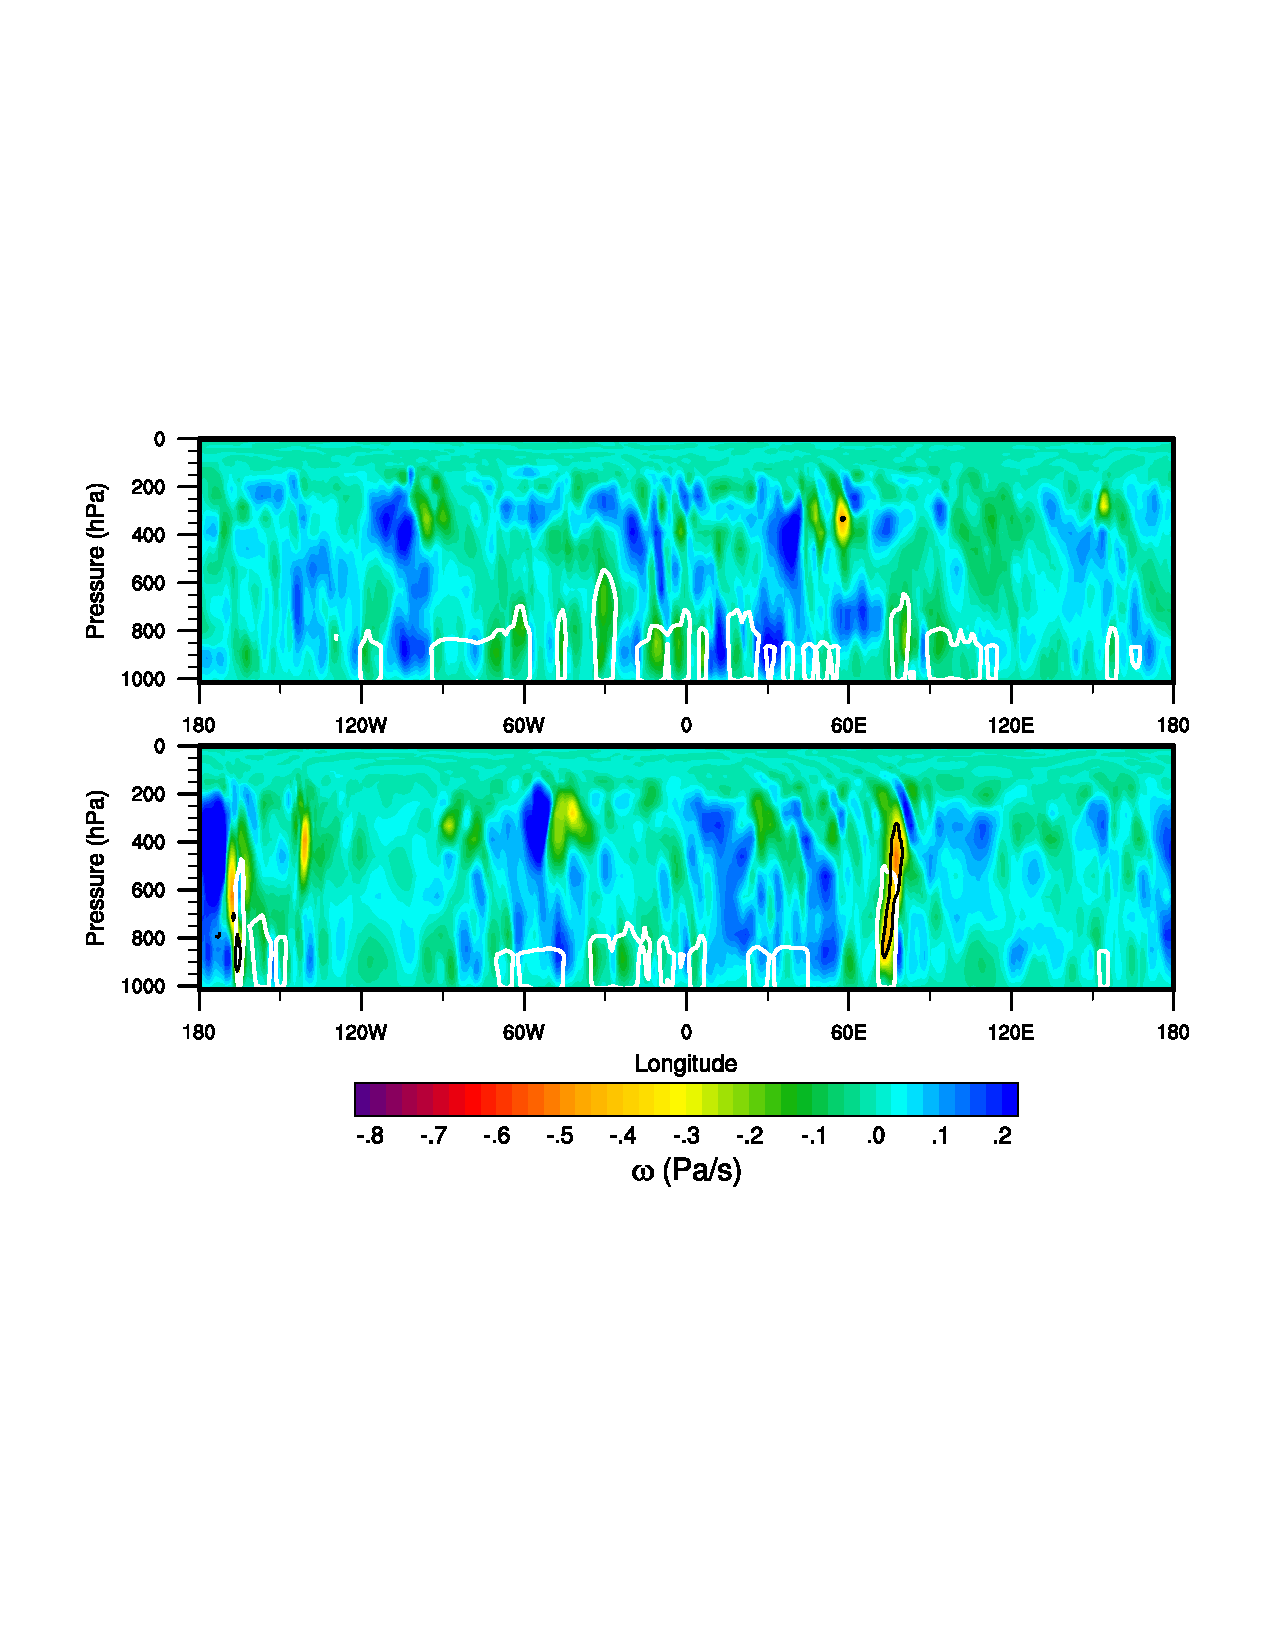
\includegraphics[width=20pc,angle=0]{figs/temp_trans.pdf}\\
\end{center}
\caption{(a,b) Two snapshots of $\omega$ for a longitude-pressure transect at $\sim 18^{\circ}$ latitude in the $ne30$ simulation, overlain by the $0.0075$ kg/m$^2$/s contour of the ZM mass flux (white) delineating the region where the ZM scheme is active, and the 15 K/day contour of the total physics tendencies (black), indicating stratiform cloud formation.}
\label{fig:transect}
\end{figure}

Figure~\ref{fig:cape-subt} shows the dilute CAPE values computed from mean temperature and moisture of subsiding and ascending regions in the $\pm \left( 10^{\circ}-30^{\circ} \right)$ latitude bands, hereafter referred to as the subtropics. The spread in dilute CAPE between ascending and descending grid columns is much smaller than for the deep tropics (Figure~\ref{fig:cape}a), and the dilute CAPE computed from the mean temperature and moisture over the entire subtropics varies much less with resolution compared with the deep tropics ($\sim 20$ J/kg across all resolutions, compared with $\sim 80$ J/kg across resolutions in the deep tropics). Also unlike the deep tropics, the reduction in dilute CAPE with resolution is not from an increase in occurrence of subsiding grid columns, since the space-time weights of ascending/descending motion are more-or-less invariant with resolution (Figure~\ref{fig:cape-subt}b). The decline in dilute CAPE with resolution in the subtropics is a result of increased stability due to changes in environmental temperature from the larger magnitude downward motion (not shown). This increased stability with resolution is not sufficient to overcome the large latent heat fluxes and mitigate the shallow convection regime of the ZM scheme, consistent with the local minimum in the R-values from the logistic regression in drizzling regions (Figure~\ref{fig:4zonal}a).

\begin{figure}
\begin{center}
\noindent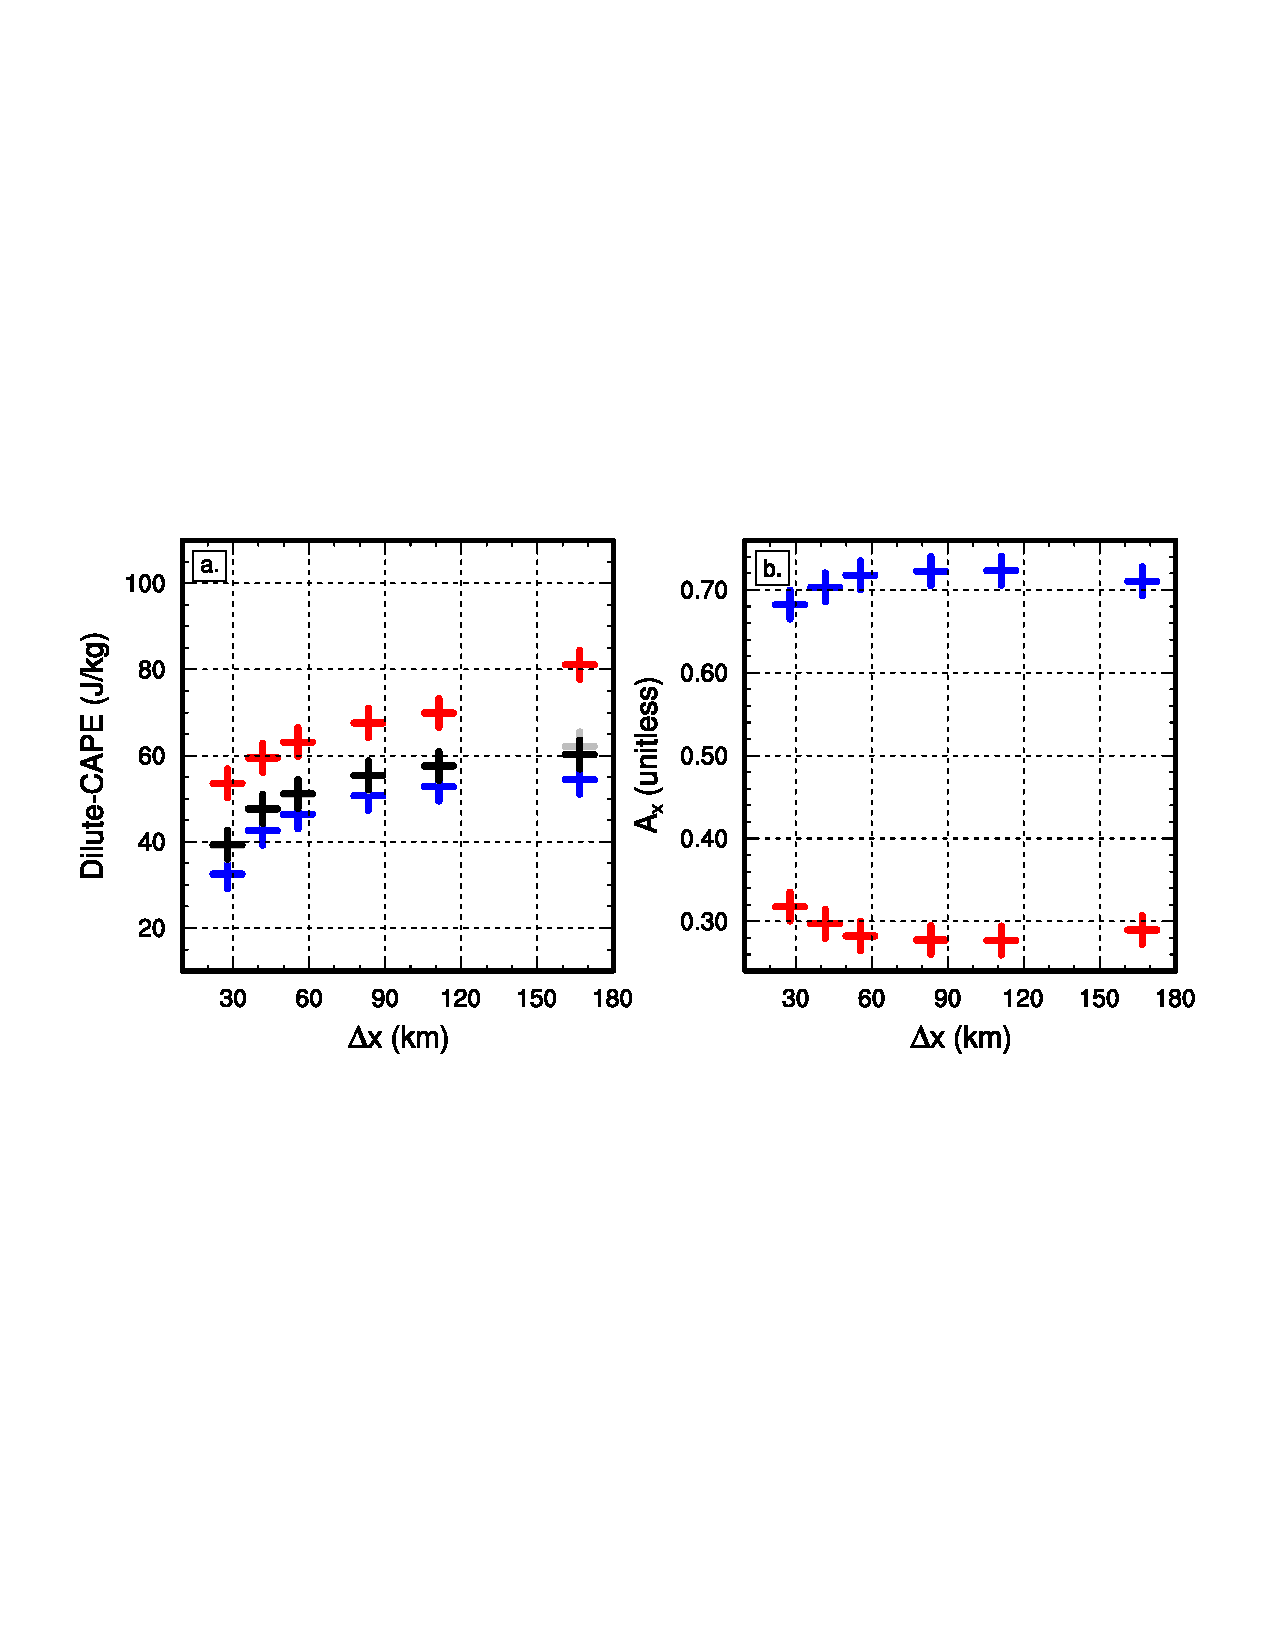
\includegraphics[width=20pc,angle=0]{figs/temp_cape-subtropics.pdf}\\
\end{center}
\caption{(a) Dilute CAPE computed from time mean temperature and moisture profiles of ascending (red), subsiding (blue) and all grid columns (black) in the subtropics ($\pm \left(10^{\circ}-30^{\circ} \right)$ latitude bands), and (b) space-time weights of ascending (red) and descending (blue) grid columns in the subtropics. Grey crosses in (a) are dilute CAPE derived from the sum of the products of space-time weights with the dilute CAPE values of ascending/descending grid columns.}
\label{fig:cape-subt}
\end{figure}

\subsection{Vertical Velocities and Stratiform Precipitation}

In contrast to the impact of vertical motion on the ZM scheme, the stratiform scheme is more intuitively connected to vertical velocities. \cite{RETAL2016CD} proposed that total precipitation rates in models ($R$, sum of convective and stratiform precipitation rates) are determined by the upward moisture flux through cloud base,
\begin{equation}
R \approx -\frac{1}{g\rho_{w}} \omega^+ q^+ \label{eq:mflux}
\end{equation}
where $\omega^+$ and $q^+$ are the upward $\omega$ and specific humidity $q$ at cloud base, respectively, and $\rho_w$ is the density of rainwater. 

Through approximating the cloud base as the $850$ hPa level, equation~\ref{eq:mflux} was found to be a good approximation to total precipitation rates in a regional model \citep{RETAL2016CD} and in the CAM-SE AGCM with CAM5 physics \citep{OETAL2016JAMES}. Figure~\ref{fig:mflux} shows the median convective, stratiform and total precipitation rates conditioned on the $850$ hPa moisture flux using $1$ mm/day bins, in the CAM6 $ne30$ simulation. The figure shows that the moisture flux is a good approximation to the median total precipitation rate, and that the increase in precipitation rates with moisture flux is primarily from the stratiform precipitation scheme. 

\begin{figure}
\begin{center}
\noindent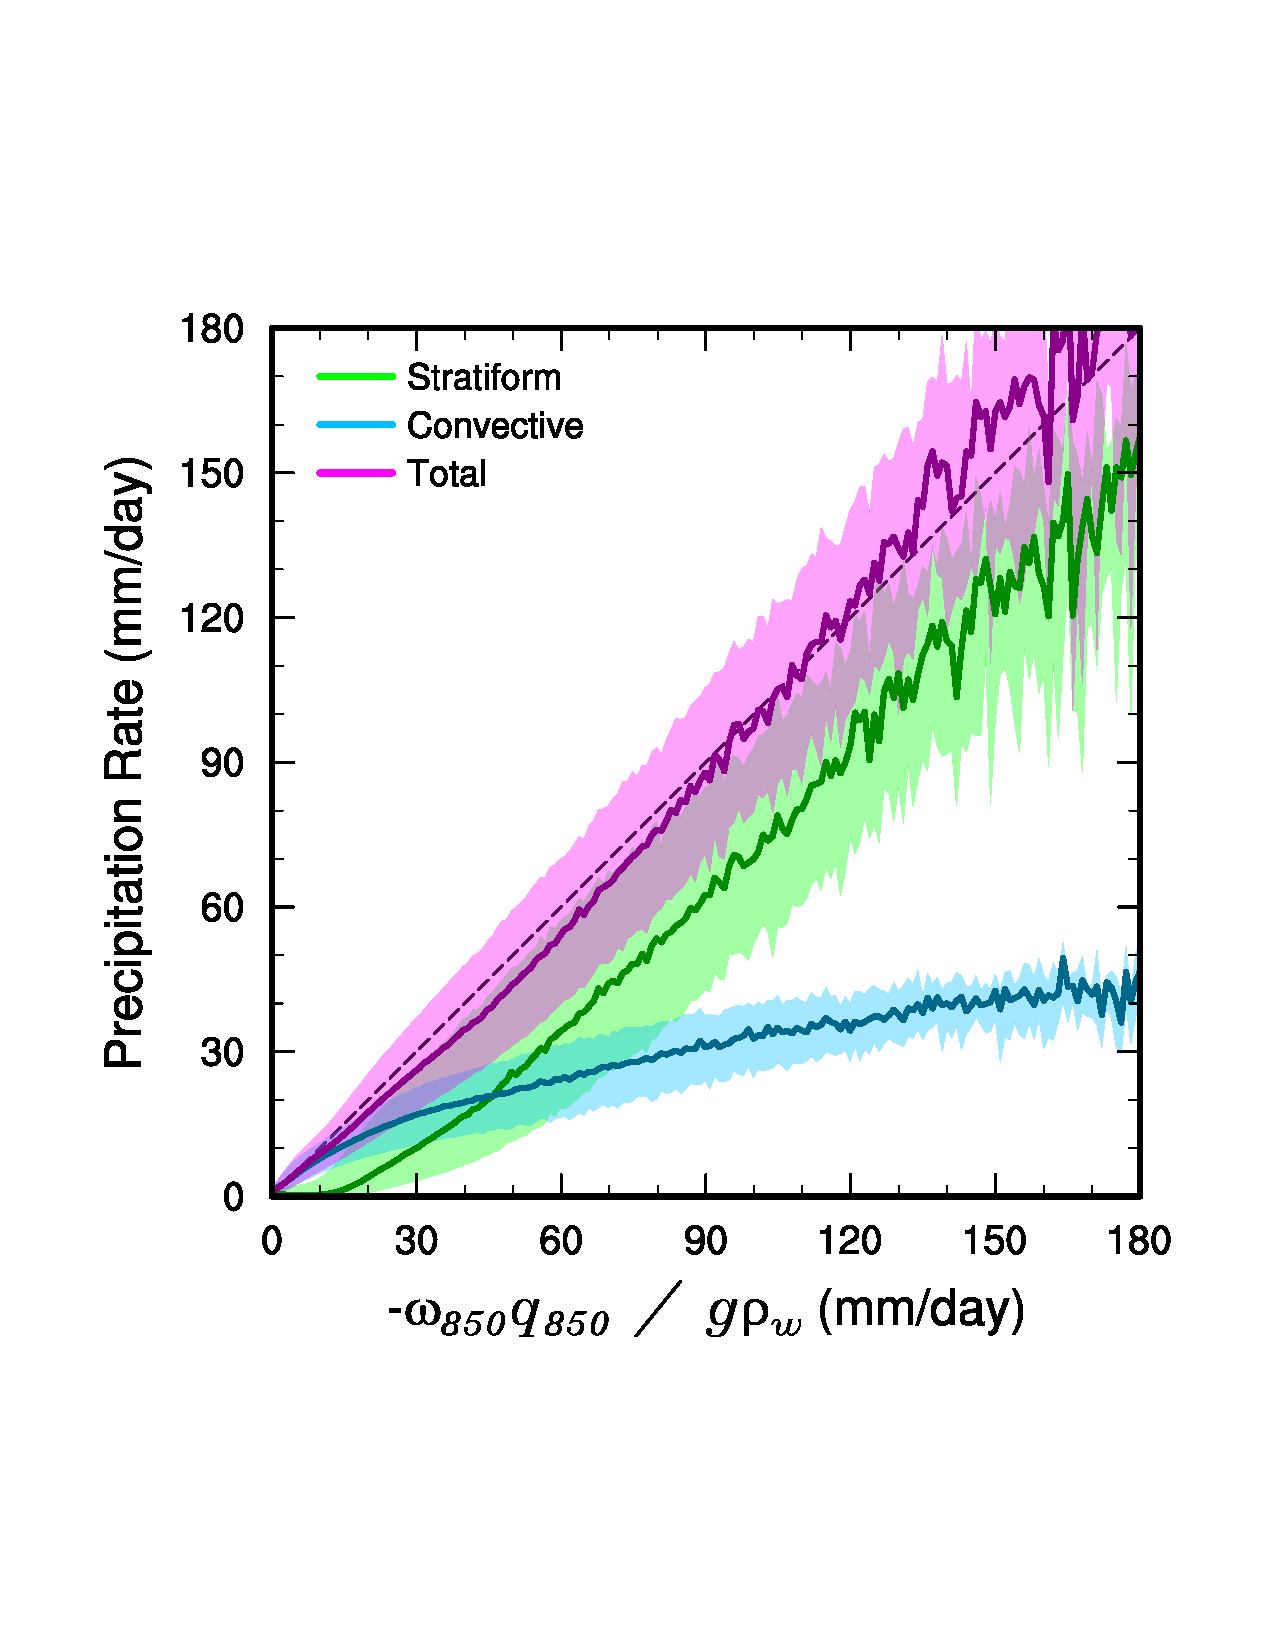
\includegraphics[width=20pc,angle=0]{figs/temp_mflux.pdf}\\
\end{center}
\caption{Precipitation rates vs. upward moisture flux at the 850 hPa level. Solid lines refer to median stratiform (green), convective (blue) and total (magenta) precipitation rates conditional on bins of the moisture flux, and shaded regions refer to the conditional interquartile ranges.}
\label{fig:mflux}
\end{figure}

The increase in stratiform precipitation rates with resolution is likely due to the increase in magnitude of $\omega$ with resolution. To unravel the contributions of $\omega$ and $q$ at the 850 hPa level, $\omega_{850}$ and $q_{850}$ to the increase in climatological stratiform precipitation with resolution, the area averaged, climatological stratiform precipitation rate $\overline{R_{s}}$ can be decomposed into a double sum of the product of the time mean magnitude $M_s$ and time mean spatial frequency $f_s$, over $\omega_{850}$ and $q_{850}$ space,
\begin{equation}
\overline{R_{s}} = \sum_i \sum_j f_s \left( \omega_i , q_j \right) M_s \left( \omega_i , q_j \right) \label{eq:pdecomp}
\end{equation}
after \cite{TETAL2018CD}, and the subscript $850$ is dropped from $\omega$ and $q$ for brevity. 

Table~\ref{tbl:table2} indicates that the $\pm 15^{\circ}$ latitude band accounts for most of the change in global mean stratiform precipitation with resolution, and so $\overline{R_s}$ is defined as the mean over the $\pm 15^{\circ}$ latitude region. Figure~\ref{fig:pdecomp} is a plot of the terms $M_s \left( \omega_i , q_j \right)$ and $f_s \left( \omega_i , q_j \right) M_s \left( \omega_i , q_j \right)$ for all resolutions,. The plots are computed using 6-hourly instantaneous output of $\omega_{i}$ and $q_{j}$, with 0.05 Pa/s and 0.4 g/kg bins. Values in  $\left( \omega_{i} , q_{j} \right)$ space are only shown for bins with $f_s \geq1 \times 10^{-5}$, a reasonable cut-off to a bins' contribution to $\overline{R_s}$. The $M_s$ plots show that larger magnitude $\omega_{850}$ correspond to larger magnitude time-mean stratiform precipitation rates, and these larger precipitation rates are associated with larger spatial frequencies $f_s \left( \omega_i , q_j \right)$ at higher resolutions. These large magnitude stratiform precipitation rates increasingly contribute to the increase in $\overline{R_{s}}$ with resolution, as seen by the expansion of $f_s \left( \omega_i , q_j \right) M_s \left( \omega_i , q_j \right)$ to include larger magnitude $\omega_{850}$. Changes to the time mean spatial frequency of the $q_{850}$ field contributes comparatively much less to changes in stratiform precipitation.

\begin{figure}
\begin{center}
\noindent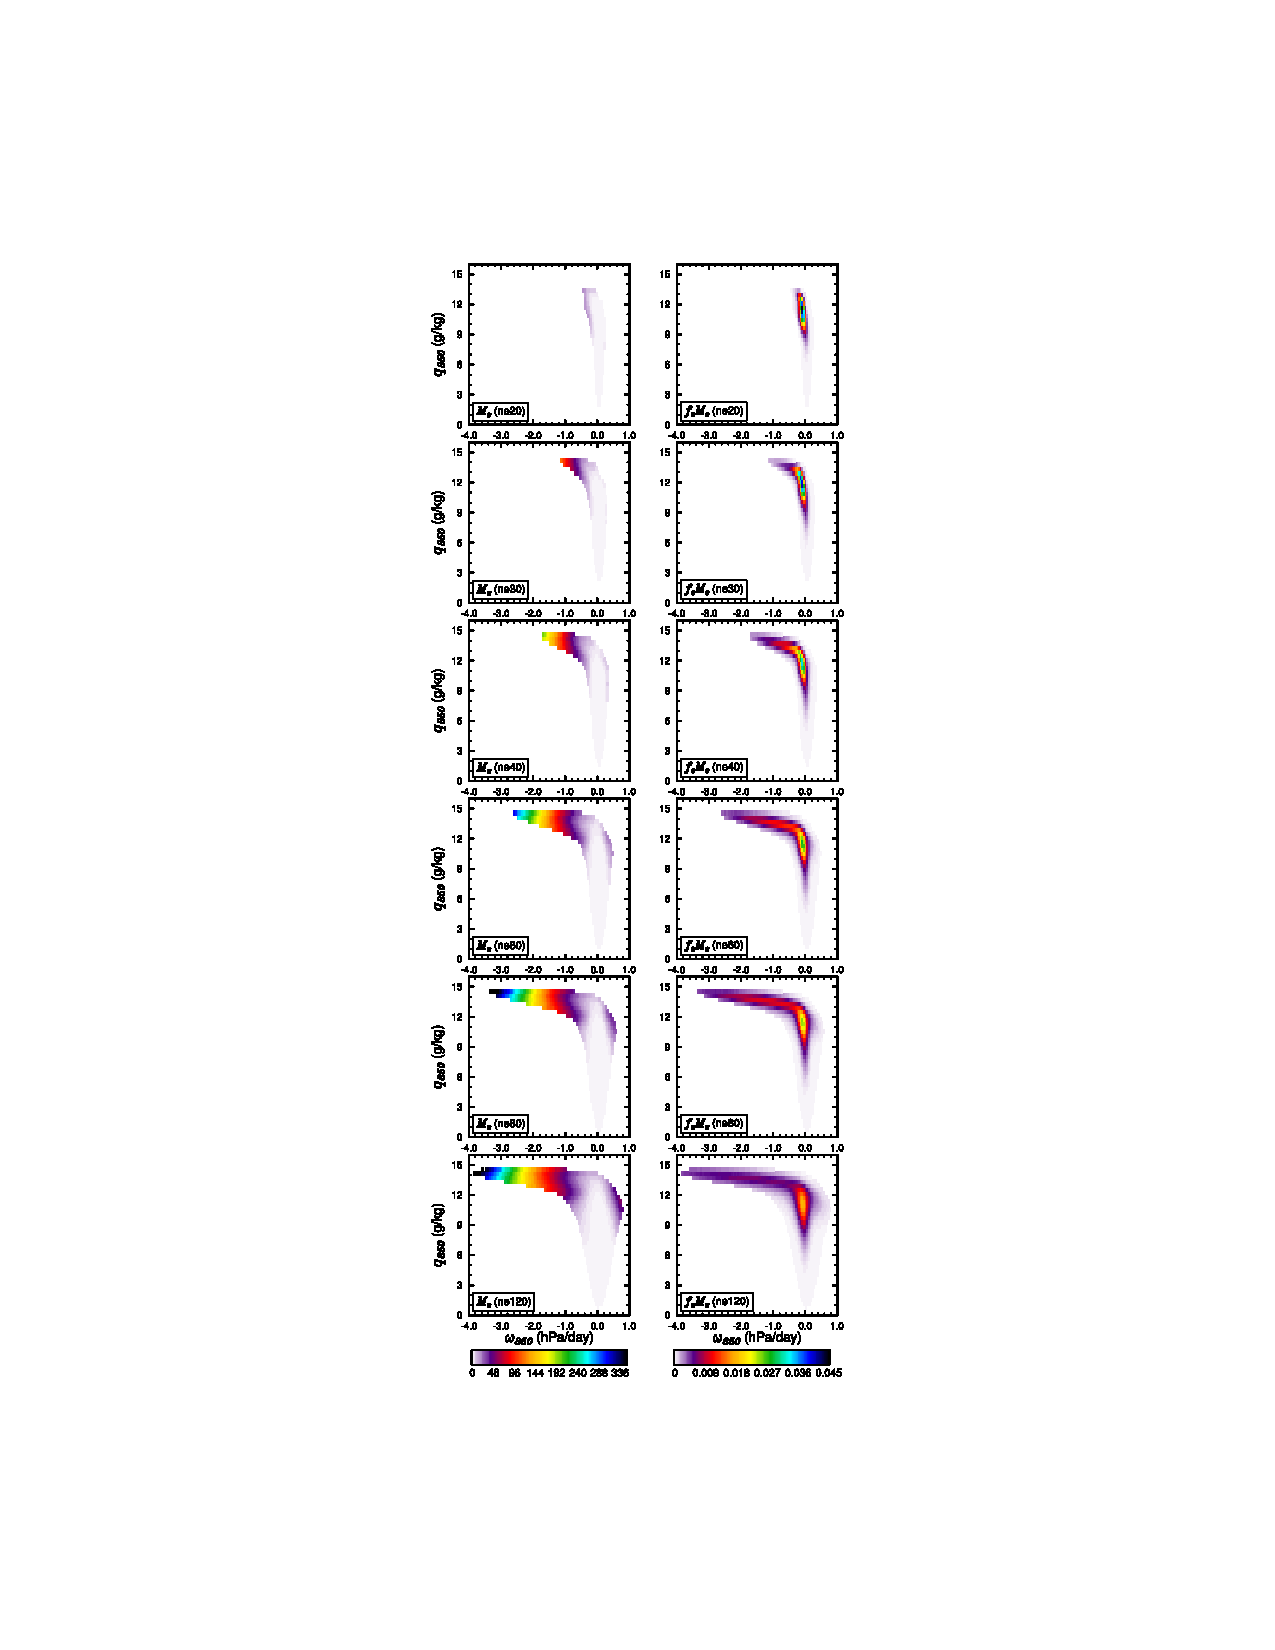
\includegraphics[width=20pc,angle=0]{figs/temp_pdecomp.pdf}\\
\end{center}
\caption{Decomposition of the climatological stratiform precipitation rates, averaged over the $\pm 15^{\circ}$ latitude band into $\omega_{850}$ and $q_{850}$ environmental conditions. Left column shows the time mean magnitude term $M\left( \omega_i , q_j \right)$ and the right column is the magnitude term multiplied by the space-time frequency term $f\left( \omega_i , q_j \right) \times M\left( \omega_i , q_j \right)$. Integrals over $f \times M$ gives the climatological, area averaged stratiform precipitation rate. Panel labels denote the grid resolution of the model run.}
\label{fig:pdecomp}
\end{figure}

\section{Conclusions}

%In the $\pm 10^{\circ}$ latitude band, the deep tropics, there is a reduction in the occurrence of ascending grid columns with resolution, which drives an increase in occurrence of subsiding regions. The reduction in occurrence of ascending motion in the deep tropics with resolution likely manifests as a reduction in the area of resolved updrafts with resolution, since the horizontal scale of large buoyancy stratiform clouds collapse to smallest resolvable feature in the model \citep{HR2018JAMES}, i.e., the models effective resolution. The PDF's of vertical velocities indicate that it is this resolution dependence of stratiform clouds that sets a power law relationship of the magnitude of the vertical velocities with resolution $\Delta x^{n}$, with $n=-1$. This scaling also indicates that for a doubling of the resolution, the same upward mass flux can be achieved in the half the area, and so it seems plausible that the reduction in the occurrence of ascending motion with resolution is also a result of the greater efficiency of the resolved mass fluxes with resolution.

\ack 
Funding support for this work was in part provided by the U.S. Department of Energy Office of Science (DE-SC0019459) and the National Science Foundation (AGS1648629). Computing and data storage resources, including the Cheyenne supercomputer (doi:10.5065/D6RX99HX), were provided by the Computational and Information Systems Laboratory (CISL) at the National Center for Atmospheric Research (NCAR). Herrington would like to thank Dr. Sultan Hameed for his assistance with the statistical analysis used in this study.

\bibliographystyle{wileyqj}
\bibliography{bib}
\end{document}
